\chapter{Topologische Grundbegriffe}
\section{Topologische Räume}
\begin{definition}\xindex{Raum!topologischer}\xindex{Menge!offene}\xindex{Menge!abgeschlossene}%
    Ein \textbf{topologischer Raum} ist ein Paar $(X, \fT)$ bestehend
    aus einer Menge $X$ und $\fT \subseteq \powerset{X}$ mit
    folgenden Eigenschaften
    \begin{defenumprops}
        \item $\emptyset, X \in \fT$
        \item \label{def:topologie.ii} Sind $U_1, U_2 \in \fT$, so ist $U_1 \cap U_2 \in \fT$
        \item Ist $I$ eine Menge und $U_i \in \fT$ für jedes $i \in I$,
              so ist $\displaystyle \bigcup_{i \in I} U_i \in \fT$
    \end{defenumprops}
    Die Elemente von $\fT$ heißen \textbf{offene Teilmengen} von $X$. 

    $A \subseteq X$ heißt \textbf{abgeschlossen}, wenn $X \setminus A$ offen ist.
\end{definition}

Es gibt auch Mengen, die weder abgeschlossen, noch offen sind wie z.~B. $[0,1)$.
Auch gibt es Mengen, die sowohl abgeschlossen als auch offen sind.

\begin{bemerkung}[Mengen, die offen \& abgeschlossen sind, existieren]%
    Betrachte $\emptyset$ und $X$ mit der \enquote{trivialen Topologie}
    \xindex{Topologie!triviale}\index{Klumpentopologie|see{triviale Topologie}} $\fT_{\ts{triv}} = \Set{\emptyset, X}$.

    Es gilt: $X \in \fT$ und $\emptyset \in \fT$, d.~h. $X$ und $\emptyset$
    sind offen. Außerdem $X^C = X \setminus X = \emptyset \in \fT$
    und $X \setminus \emptyset = X \in \fT$, d.~h. $X$ und $\emptyset$
    sind als Komplement offener Mengen abgeschlossen.$\qed$
\end{bemerkung}

\begin{beispiel}[Topologien]
    \begin{enumerate}[label=\arabic*)]
        \item $X = \mdr^n$ mit der euklidischen Metrik. \xindex{Topologie!euklidische}
              \begin{align*}
                U \subseteq \mdr^n \text{ offen} \gdw\;&\text{für jedes $x \in U$ gibt es $r > 0$,}\\
                                                       &\text{sodass $\fB_r(x) = \Set{y \in \mdr^n | d(x,y) < r} \subseteq U$}
              \end{align*}
              Diese $\fB$ Topologie wird auch \enquote{Standardtopologie des $\mdr^n$}\xindex{Standardtopologie} genannt.
              Sie beinhaltet unter anderem alle offenen Kugeln, aber
              z.~B. auch Schnitte zweier Kugeln mit unterschiedlichem
              Mittelpunkt (vgl. \cref{def:topologie.ii}).
        \item Jeder metrische Raum $(X, d)$ ist auch ein topologischer Raum.
        \item Für eine Menge $X$ heißt $\fT = \powerset{X}$ \enquote{diskrete Topologie}\xindex{Topologie!diskrete}.
        \item $X :=\mdr, \fT_Z := \Set{U \subseteq \mdr | \mdr \setminus U \text{ endlich}} \cup \Set{\emptyset}$ heißt \enquote{Zariski-Topologie} \xindex{Topologie!Zariski}\\
              Beobachtungen: 
            \begin{itemize}
                \item $U \in \fT_Z \gdw \exists f \in \mdr[X]$, sodass $\mdr \setminus U = V(f) = \Set{x \in \mdr | f(x) = 0}$
                \item Es gibt keine disjunkten offenen Mengen in $\fT_Z$.
            \end{itemize}
        \item $X := \mdr^n, \fT_Z = \{U \subseteq \mdr^n | \text{Es gibt Polynome } f_1, \dots, f_r \in \mdr[X_1, \dots, X_n] \text{ sodass }\\\mdr^n \setminus U = V(f_1, \dots, f_r)\}$
        \item $X := \Set{0,1}, \fT = \Set{\emptyset, \Set{0,1}, \Set{0}}$ heißt \enquote{Sierpińskiraum}.\xindex{Sierpińskiraum}\\
              $\emptyset, \Set{0,1}, \Set{1}$ sind dort alle abgeschlossenen Mengen.
    \end{enumerate}
\end{beispiel}

\begin{definition}\xindex{Umgebung}%
    Sei $(X, \fT)$ ein topologischer Raum und $x \in X$.

    Eine Teilmenge $U \subseteq X$ heißt \textbf{Umgebung} von $x$,
    wenn es ein $U_0 \in \fT$ gibt mit $x \in U_0$ und $U_0 \subseteq U$.

    Gilt eine Eigenschaft in einer Umgebung, so sagt man, dass die Eigenschaft
    \textbf{lokal}\xindex{lokal} gilt.
\end{definition}

\begin{definition}%
    Sei $(X, \fT)$ ein topologischer Raum und $M \subseteq X$ eine Teilmenge.
    \begin{defenum}
        \item $\displaystyle M^\circ := \Set{x \in M | M \text{ ist Umgebung von } x} = \bigcup_{\overset{U \subseteq M} {U \in \fT}} U $ heißt \textbf{Inneres} oder \textbf{ offener Kern} von $M$. \xindex{Inneres} \xindex{Kern!offener}
        \item $\displaystyle \overline{M} := \bigcap_{\mathclap{\overset{M \subseteq A}{A \text{ abgeschlossen}}}} A$ heißt \textbf{abgeschlossene Hülle} oder \textbf{Abschluss} von $M$. \xindex{Abschluss}
        \item $\partial M := \overline{M} \setminus M^\circ$ heißt \textbf{Rand} von $M$. \xindex{Rand}
        \item $M$ heißt \textbf{dicht} in $X$, wenn $\overline{M} = X$ ist. \xindex{dicht}
    \end{defenum}
\end{definition}

\begin{beispiel}
    \begin{bspenum}
        \item Sei $X = \mdr$ mit euklidischer Topologie und 
              $M = \mdq$. Dann gilt: $\overline{M} = \mdr$ und 
              $M^\circ = \emptyset$
        \item Sei $X = \mdr$ und $M=(a,b)$. Dann gilt: 
              $\overline{M} = [a,b]$
        \item Sei $X = \mdr, \fT = \fT_Z$ und $M = (a,b)$. Dann gilt:
              $\overline{M} = \mdr$
    \end{bspenum}
\end{beispiel}

\begin{definition}\xindex{Basis}\xindex{Subbasis}%
    Sei $(X, \fT)$ ein topologischer Raum.
    \begin{defenum}
        \item $\fB \subseteq \fT$ heißt \textbf{Basis} der Topologie $\fT$,
              wenn jedes $U \in \fT$ Vereinigung von Elementen aus $\fB$
              ist.
        \item $\calS \subseteq \fT$ heißt \textbf{Subbasis} der Topologie $\fT$, wenn jedes
              $U \in \fT$ Vereinigung von endlichen Durchschnitten
              von Elementen aus $\calS$ ist.
    \end{defenum}
\end{definition}

\begin{beispiel}
    \begin{bspenum}
        \item Gegeben sei $X = \mdr^n$ mit euklidischer Topologie $\fT$. Dann ist
              \[\fB = \Set{B_r(x) | r \in \mdq_{> 0}, x \in \mdq^n}\]
              ist eine abzählbare Basis von $\fT$.
        \item Sei $(X, \fT)$ ein topologischer Raum mit 
              $X = \Set{0,1,2}$ und $\fT = \Set{\emptyset, \Set{0}, \Set{0,1}, X}$.\\
              Dann ist $\calS = \Set{\emptyset, \Set{0,1}, \Set{0,2}}$ eine Subbasis von 
              $\fT$, da gilt:
              \begin{itemize}
                \item $\emptyset \in \calS$
                \item $\Set{0} = \Set{0, 1} \cap \Set{0,2}$
                \item $\Set{0,1} \in \calS$
                \item $X = \Set{0,1} \cup \Set{0,2}$
              \end{itemize}
              Allerings ist $\calS$ keine Basis von $(X, \fT)$, da
              $\Set{0}$ nicht als Vereinigung von Elementen aus $\calS$
              erzeugt werden kann.
    \end{bspenum}
\end{beispiel}

\begin{bemerkung}
    Sei $X$ eine Menge und $\calS \subseteq \powerset{X}$. Dann gibt es
    genau eine Topologie $\fT$ auf $X$, für die $\calS$ Subbasis ist.
\end{bemerkung}

\begin{definition}\xindex{Spurtopologie|see{Teilraumtopologie}}\xindex{Teilraum}\xindex{Teilraumtopologie}\xindex{Unterraumtopologie|see{Teilraumtopologie}}%
    Sei $(X, \fT)$ ein topologischer Raum und $Y \subseteq X$.\\
    $\fT_Y := \Set{U \cap Y | U \in \fT}$ ist eine Topologie auf $Y$.

    $\fT_Y$ heißt \textbf{Teilraumtopologie} und $(Y, \fT_Y)$ heißt ein 
    \textbf{Teilraum} von $(X, \fT)$.
\end{definition}

Die Teilraumtopologie wird auch \textit{Spurtopologie} oder 
\textit{Unterraumtopologie} genannt.

%%%%%%%%%%%%%%%%%%%%%%%%%%%%%%%%%%%%%%%%%%%%%%%%%%%%%%%%%%%%%%%%%%%%%
% Mitschrieb vom 24.10.2013                                         %
%%%%%%%%%%%%%%%%%%%%%%%%%%%%%%%%%%%%%%%%%%%%%%%%%%%%%%%%%%%%%%%%%%%%%
\begin{definition}\xindex{Produkttopologie}%
    Seien $X_1, X_2$ topologische Räume.\\
    $U \subseteq X_1 \times X_2$ sei offen, wenn es zu jedem $x = (x_1, x_2) \in U$
    Umgebungen $U_i$ um $x_i$  mit $i=1,2$ gibt, sodass $U_1 \times U_2 \subseteq U$
    gilt.

    $\fT = \Set{U \subseteq X_1 \times X_2 | U \text{ offen}}$
    ist eine Topologie auf $X_1 \times X_2$. Sie heißt \textbf{Produkttopologie}.
    $\fB = \Set{U_1 \times U_2 | U_i \text{ offen in } X_i, i=1,2}$
    ist eine Basis von $\fT$.
\end{definition}

\begin{figure}[htp]
    \centering
    \documentclass[varwidth=true, border=2pt]{standalone}
\usepackage{tikz}
\usepackage{pgfplots}

\begin{document}
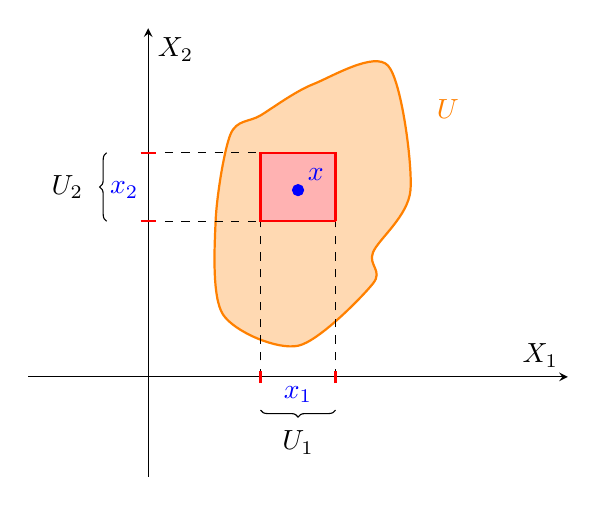
\begin{tikzpicture}
    \begin{axis}[
        axis x line=middle,
        axis y line=middle,
        %width=9cm,
        %height=4.5cm,
        xmin=-1,     % start the diagram at this x-coordinate
        xmax= 5,    % end   the diagram at this x-coordinate
        ymin=-1,     % start the diagram at this y-coordinate
        ymax= 5,   % end   the diagram at this y-coordinate
        xlabel=$X_1$,
        ylabel=$X_2$,
        ticks=none,
        enlargelimits=true,
        after end axis/.code={
            \draw [decorate,decoration={brace,mirror,raise=15pt}] (axis cs:0,3.6) -- (axis cs:0,2.5) node [midway,left=20pt] {$U_2$};
            \draw [decorate,decoration={brace,mirror,raise=12pt}] (axis cs:1.5,0) -- (axis cs:2.5,0) node [midway,below=16pt] {$U_1$};
        }]

        \addplot[mark=none, orange, smooth cycle, thick, fill=orange!30] coordinates {(1,1) (2,0.5) (3,1.5) (3,2) (3.5,3) (3.2, 5) (2.2, 4.7) (1.5, 4.2) (1.1, 3.9) (0.9, 2.5)};
        \node[orange] at (axis cs:4,4) [anchor=south] {$U$};

        % Draw help lines
        \addplot[dashed] coordinates {(1.5,0) (1.5,3.6)};
        \addplot[dashed] coordinates {(2.5,0) (2.5,3.6)};
        \addplot[dashed] coordinates {(0,2.5) (2.5,2.5)};
        \addplot[dashed] coordinates {(0,3.6) (2.5,3.6)};

        % Draw solid square
        \addplot[mark=none, red, thick, fill=red!30] coordinates {(2.5,2.5) (2.5,3.6) (1.5,3.6) (1.5,2.5) (2.5,2.5)};

        % Draw x and annotation
        \node[blue] at (axis cs:2,3) [anchor=south west] {$x$};
        \addplot[mark=*, blue] coordinates {(2,3)};

        % Draw ticks of help lines
        \addplot[mark=none, red, thick] coordinates {(1.5, -0.1) (1.5,0.1)};
        \addplot[mark=none, red, thick] coordinates {(2.5, -0.1) (2.5,0.1)};
        \addplot[mark=none, red, thick] coordinates {(-0.1, 2.5) (0.1,2.5)};
        \addplot[mark=none, red, thick] coordinates {(-0.1, 3.6) (0.1,3.6)};

        % Draw axis text
        \node[blue] at (axis cs:0,3) [anchor=east] {$x_2$};
        \node[blue] at (axis cs:2,0) [anchor=north] {$x_1$};

    \end{axis}
\end{tikzpicture}
\end{document}

    \caption{Zu $x=(x_1, x_2)$ gibt es Umgebungen $U_1, U_2$ mit $U_1 \times U_2 \subseteq U$}
\end{figure}

\begin{beispiel}[Produkttopologien]
    \begin{bspenum}
        \item $X_1 = X_2 = \mdr$ mit euklidischer Topologie.\\
              $\Rightarrow$ Die Produkttopologie auf $\mdr \times \mdr = \mdr^2$
              stimmt mit der euklidischen Topologie auf $\mdr^2$ überein.
        \item $X_1 = X_2 = \mdr$ mit Zariski-Topologie.
              $\fT$ Produkttopologie auf $\mdr^2$: $U_1 \times U_2$\\
              (Siehe \cref{fig:zariski-topologie})
    \end{bspenum}

    \begin{figure}[htp]
        \centering
        \documentclass[varwidth=true, border=2pt]{standalone}
\usepackage{tikz}
\usepackage{pgfplots}
\usepackage{amsmath,amssymb}

\begin{document}
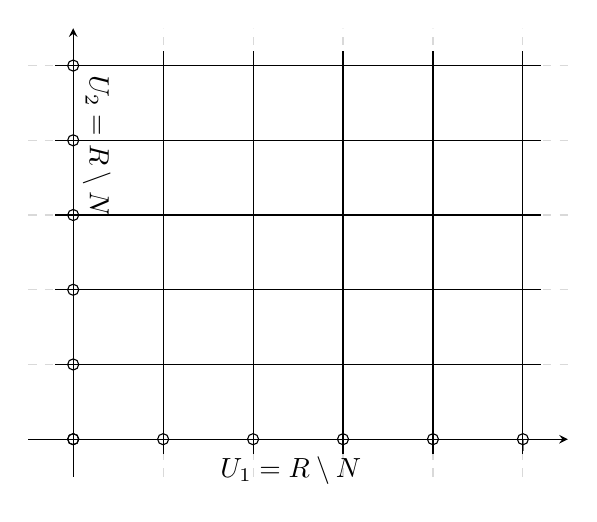
\begin{tikzpicture}
    \begin{axis}[
        axis x line=middle,
        axis y line=middle,
        grid = major,
        grid style={dashed, gray!30},
        xmin= 0,     % start the diagram at this x-coordinate
        xmax= 5,    % end   the diagram at this x-coordinate
        ymin= 0,     % start the diagram at this y-coordinate
        ymax= 5,   % end   the diagram at this y-coordinate
        xtick={-1,0,1,2,3,4,5},
        ytick={-1,0,1,2,3,4,5},
        xlabel={$U_1 = \mathbb{R} \setminus \mathbb{N}$},
        xlabel style={xshift=-2.5cm,yshift=-0.7cm},
        ylabel={$U_2 = \mathbb{R} \setminus \mathbb{N}$},
        ylabel style={rotate=-90, xshift=1.5cm},
        xticklabels={,,},
        yticklabels={,,},
        tick align=outside,
        enlargelimits=true]


        % Draw solid square
        \addplot[mark=o] coordinates {(0,0) (1,0) (2,0) (3,0) (4,0) (5,0)};
        \addplot[mark=o] coordinates {(0,0) (0,1) (0,2) (0,3) (0,4) (0,5)};

        \foreach \i in {0,1,2,3,4,5} {
            \addplot[mark=none] coordinates {(-0.2,\i) (5.2,\i)};
            \addplot[mark=none] coordinates {(\i,-0.2) (\i,5.2)};
        }
        \addplot[mark=none] coordinates {(0,2) (5,2)};
    \end{axis}
\end{tikzpicture}
\end{document}

        \caption{Zariski-Topologie auf $\mdr^2$}
        \label{fig:zariski-topologie}
    \end{figure}
\end{beispiel}

\begin{definition}\xindex{Quotiententopologie}%
    Sei $X$ ein topologischer Raum, $\sim$ eine Äquivalenzrelation auf $X$,
    $\overline{X} = X /_\sim$ sei die Menge der Äquivalenzklassen,
    $\pi: x \rightarrow \overline{x}, \;\;\; x \mapsto [x]_\sim$.

    \[\fT_{\overline{X}} := \Set{U \subseteq \overline{X} | \pi^{-1}(U) \in \fT_X}\]

    $(\overline{X}, \fT_{\overline{X}})$ heißt \textbf{Quotiententopologie}.
\end{definition}

\begin{beispiel}
    $X = \mdr, a \sim b :\Leftrightarrow a-b \in \mdz$
    
    \documentclass[varwidth=true, border=2pt]{standalone}
\usepackage{amsmath,amssymb}
\usepackage{pgfplots}
\usepackage{tikz}
\usepackage{tkz-fct}
\usetikzlibrary{shapes.misc}

\begin{document}
\tikzset{
    point/.style={
        thick,
        draw=gray,
        cross out,
        inner sep=0pt,
        minimum width=4pt,
        minimum height=4pt,
    },
}
\begin{tikzpicture}
  
  \draw[->] (-1.5,0) -- (5.5,0) node [below] {$\mathbb{R}$};

  \foreach \x in {-1,...,5}
    \draw (\x,0.1) -- (\x,-0.1) node [below] {\x};

  \foreach \x in {-1,...,4} {
    \draw[red] (\x+0.6,0.01) -- (\x+0.6,-0.14) node [below] {};
    \draw[red] (\x+1.2,0.01) -- (\x+1.2,-0.14) node [below] {};
    \draw[red] (\x+0.6,-0.07) -- (\x+1.2,-0.07) node [below] {};
    }

    \begin{scope}[shift={(0,-2)}]
        \draw[thick] (0cm,0cm) circle(1cm);
        \draw[thick, red] ([shift={(216:1cm)}]-0.0,0) arc (216:-72:1cm);
        \draw (0:1cm) node[point, label={[right]{$0$}}] {};
        \path node[point, blue, label={[blue,above]{$\overline{a}$}}] (posU) at (-252:1cm) {};
        \path node[label={[red,left]{$U$}}] at (30:1cm) {};
    \end{scope}
    \draw (3.7cm,0cm) node[point, blue, label={[blue,above]{$a$}}] (posA) {};
    \draw (0.7cm,0cm) node[point, blue, label={[blue,above]{$\pi^{-1}(u)$}}] {};
    \draw[dashed, blue, thick] plot [smooth] coordinates{(posU) (0.2,-0.8) (2.5,-1) (posA)};

    \draw[blue, dashed, thick] (3.7cm,0cm) arc (0:180:1.5 and 0.5);

\end{tikzpicture}
\end{document}


    $0 \sim 1$, d.~h. $[0] = [1]$
\end{beispiel}

\begin{beispiel}\xindex{Torus}
    Sei $X = \mdr^2$ und $(x_1, y_1) \sim (x_2, y_2) \gdw x_1 - x_2 \in \mdz$ 
    und $y_1 - y_2 \in \mdz$. Dann ist $X /_\sim$ ein Torus.
\end{beispiel}

\begin{beispiel}[Projektiver Raum]\xindex{Raum!projektiver}%
    \begin{align*}
        X= \mdr^{n+1} \setminus \Set{0},\;\;\; x \sim y &\gdw \exists \lambda \in \mdr^\times \text{ mit } y = \lambda x\\
            &\gdw x \text{ und } y \text{ liegen auf der gleichen}\\
            &\hphantom{\gdw} \text{Ursprungsgerade}
    \end{align*}
    \[\overline{X} = \praum^n(\mdr)\]
    Also für $n=1$:\nopagebreak\\
    \begin{tikzpicture}
    \begin{axis}[
        legend pos=south east,
        axis x line=middle,
        axis y line=middle,
        %grid = major,
        width=12cm,
        height=8cm,
        %grid style={dashed, gray!30},
        xmin=-4,     % start the diagram at this x-coordinate
        xmax= 8,    % end   the diagram at this x-coordinate
        ymin=-4,     % start the diagram at this y-coordinate
        ymax= 4,   % end   the diagram at this y-coordinate
        axis background/.style={fill=white},
        %xticklabels={-2,-1.6,...,2},
        %yticklabels={-8,-7,...,8},
        %tick align=outside,
        enlargelimits=true,
        tension=0.08]
      % plot the stirling-formulae
      \addplot[domain=-4:8, red, thick,samples=500] {0.5*x}; 
      \addplot[domain=-2:2, red, thick,samples=500] {2*x}; 
      \addplot[domain=-4:8, red, thick,samples=500] {-0.5*x}; 
    \end{axis} 
\end{tikzpicture}

\end{beispiel}

\section{Metrische Räume}
\begin{definition}\xindex{Metrik}\xindex{Raum!metrischer}%
    Sei $X$ eine Menge. Eine Abbildung $d:X\times X \rightarrow \mdr_0^+$
    heißt \textbf{Metrik}, wenn gilt:

    \begin{defenumprops}
        \item Definitheit:         \tabto{4cm} $d(x,y) = 0 \gdw x = y \;\;\; \forall x, y \in X$
        \item Symmetrie:           \tabto{4cm} $d(x,y) = d(y,x) \;\;\; \forall x, y \in X$
        \item Dreiecksungleichung: \tabto{4cm} $d(x,z) \leq d(x,y) + d(y,z) \;\;\; \forall x, y, z \in X$
    \end{defenumprops}

    Das Paar $(X, d)$ heißt ein \textbf{metrischer Raum}.
\end{definition}

\begin{bemerkung}
    Sei $(X, d)$ ein metrischer Raum und
    \[\fB_r(x) := \Set{y \in X | d(x,y) < r} \text{ für } x \in X, r \in \mdr^+\]
    $\fB$ ist Basis einer Topologie auf $X$.
\end{bemerkung}

\begin{definition}\xindex{Isometrie}%
    Seien $(X, d_X)$ und $(Y, d_Y)$ metrische Räume und $\varphi: X \rightarrow Y$
    eine Abbildung mit 
    \[\forall x_1, x_2 \in X: d_X(x_1, x_2) = d_Y(\varphi(x_1), \varphi(x_2)) \]

    Dann heißt $\varphi$ eine \textbf{Isometrie} von $X$ nach $Y$.
\end{definition}

\begin{beispiel}[Skalarprodukt erzeugt Metrik]
    Sei $V$ ein euklidischer oder hermitescher Vektorraum mit Skalarprodukt
    $\langle \cdot , \cdot \rangle$.
    Dann wird $V$ durch $d(x,y) := \sqrt{\langle x-y, x-y \rangle}$ zum metrischen Raum.
\end{beispiel}

\begin{beispiel}[diskrete Metrik]\xindex{Metrik!diskrete}\xindex{Topologie!diskrete}%
    Sei $X$ eine Menge. Dann heißt
    \[d(x,y) = \begin{cases}
    0 & \text{falls } x=y\\
    1 & \text{falls } x \neq y
    \end{cases}\]
    die \textbf{diskrete Metrik}. Die Metrik $d$ induziert die 
    \textbf{diskrete Topologie}.
\end{beispiel}

\begin{beispiel}
    $X = \mdr^2$ und $d\left ((x_1, y_1), (x_2, y_2)\right ) := \max(\|x_1 - x_2\|, \|y_1 - y_2\|)$
    ist Metrik.

    \emph{Beobachtung:} $d$ erzeugt die euklidische Topologie.

    \begin{figure}[ht]
        \centering
        \subfloat[$\fB_r(0)$]{
            \documentclass[varwidth=true, border=2pt]{standalone}
\usepackage{tikz}
\usepackage{pgfplots}
\usepackage{amsmath,amssymb}

\begin{document}
\begin{tikzpicture}
    \begin{axis}[
        axis x line=middle,
        axis y line=middle,
        xmin=-1.5,     % start the diagram at this x-coordinate
        xmax= 1.5,    % end   the diagram at this x-coordinate
        ymin=-1.5,     % start the diagram at this y-coordinate
        ymax= 1.5,   % end   the diagram at this y-coordinate
        ticks=none,
        enlargelimits=true,
        after end axis/.code={
            \draw [decorate,decoration={brace,mirror,raise=2pt}] (axis cs:0,1) -- (axis cs:-1,1) node [midway,above=5pt] {$r$};
            \draw [decorate,decoration={brace,mirror,raise=2pt}] (axis cs:1,1) -- (axis cs:0,1) node [midway,above=5pt] {$r$};
            \draw [decorate,decoration={brace,mirror,raise=2pt}] (axis cs:1,0) -- (axis cs:1,1) node [midway,right=5pt] {$r$};
            \draw [decorate,decoration={brace,mirror,raise=2pt}] (axis cs:1,-1) -- (axis cs:1,0) node [midway,right=5pt] {$r$};
        }]


        % Draw solid square
        \addplot[mark=none, thick] coordinates {(-1,-1) (1,-1) (1,1) (-1,1) (-1,-1)};
        \addplot[mark=*] coordinates {(0,0)};

        % Draw axis text
        \node at (axis cs:-1,0.5) [anchor=east] {$\mathfrak{B}_r(0) = $};

    \end{axis}
\end{tikzpicture}
\end{document}

            \label{fig:open-square}
        }%
        \subfloat[Euklidische Topologie]{
            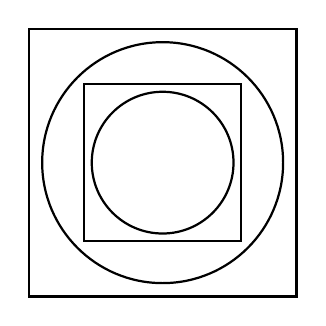
\begin{tikzpicture}[thick]
    \draw (-1,-1) -- (1,-1) -- (1,1) -- (-1,1) -- cycle;
    \draw (0cm,0cm) circle(0.9cm);

    \begin{scope}[scale=1.7]
        \draw (-1,-1) -- (1,-1) -- (1,1) -- (-1,1) -- cycle;
        \draw (0cm,0cm) circle(0.9cm);
    \end{scope}
\end{tikzpicture}

            \label{fig:quadrat-in-kreis-in-dots}
        }%
        \label{fig:metrik}
        \caption{Veranschaulichungen zur Metrik $d$}
    \end{figure}

\end{beispiel}

\begin{beispiel}[SNCF-Metrik\footnotemark]\xindex{Metrik!SNCF}
    $X = \mdr^2$ 

    \tikzset{
    point/.style={
        thick,
        draw=gray,
        cross out,
        inner sep=0pt,
        minimum width=4pt,
        minimum height=4pt,
    },
}
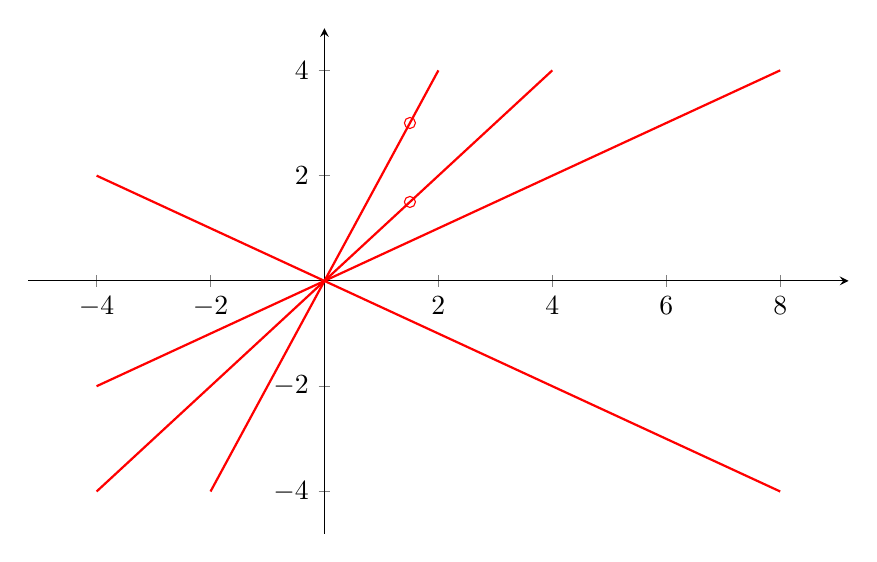
\begin{tikzpicture}
    \begin{axis}[
    legend pos=south east,
        axis x line=middle,
        axis y line=middle,
        %grid = major,
        width=12cm,
        height=8cm,
        %grid style={dashed, gray!30},
        xmin=-4,     % start the diagram at this x-coordinate
        xmax= 8,    % end   the diagram at this x-coordinate
        ymin=-4,     % start the diagram at this y-coordinate
        ymax= 4,   % end   the diagram at this y-coordinate
        axis background/.style={fill=white},
        %xticklabels={-2,-1.6,...,2},
        %yticklabels={-8,-7,...,8},
        %tick align=outside,
        enlargelimits=true,
        tension=0.08]
      % plot the stirling-formulae
      \addplot[domain=-4:8, red, thick,samples=500] {0.5*x}; 
      \addplot[domain=-2:2, red, thick,samples=500] {2*x}; 
      \addplot[domain=-4:4, red, thick,samples=500] {x}; 
      \addplot[domain=-4:8, red, thick,samples=500] {-0.5*x}; 
      \addplot[color=red,only marks,mark=o]
        plot coordinates {
            (1.5,3)
            (1.5,1.5)
        };
    \end{axis} 
\end{tikzpicture}

\end{beispiel}
\footnotetext{Diese Metrik wird auch \enquote{\href{https://de.wikipedia.org/wiki/Franz\%C3\%B6sische_Eisenbahnmetrik}{französische Eisenbahnmetrik}} genannt.}

\begin{definition}\xindex{Raum!hausdorffscher}%
    Ein topologischer Raum $X$ heißt \textbf{hausdorffsch}, wenn es
    für je zwei Punkte $x \neq y$ in $X$ Umgebungen $U_x$ um $x$
    und $U_y$ um $y$ gibt, sodass $U_x \cap U_y = \emptyset$.
\end{definition}

\begin{bemerkung}[Trennungseigenschaft]\label{Trennungseigenschaft}
    Metrische Räume sind hausdorffsch, da 
    \[d(x,y) > 0 \Rightarrow \exists \varepsilon > 0: \fB_\varepsilon(x) \cap \fB_\varepsilon(y) = \emptyset\]
\end{bemerkung}

\begin{beispiel}[Topologische Räume und Hausdorff-Räume]
    \begin{bspenum}
        \item $(\mdr, \fT_Z)$ ist ein topologischer Raum, der nicht hausdorffsch ist.
        \item $(\mdr, \fT)$ ist ein topologischer Raum, der hausdorffsch ist.
    \end{bspenum}
\end{beispiel}

\begin{bemerkung}[Eigenschaften von Hausdorff-Räumen]
    Seien $X, X_1, X_2$ Hausdorff-Räume.
    \begin{bemenum}
        \item Jeder Teilraum von $X$ ist hausdorffsch.
        \item $X_1 \times X_2$ ist hausdorffsch.
    \end{bemenum}
    \begin{figure}[htp]
        \centering
        % defining the new dimensions and parameters
\newlength{\hatchspread}
\newlength{\hatchthickness}
\newlength{\hatchshift}
\newcommand{\hatchcolor}{}
% declaring the keys in tikz
\tikzset{hatchspread/.code={\setlength{\hatchspread}{#1}},
         hatchthickness/.code={\setlength{\hatchthickness}{#1}},
         hatchshift/.code={\setlength{\hatchshift}{#1}},% must be >= 0
         hatchcolor/.code={\renewcommand{\hatchcolor}{#1}}}
% setting the default values
\tikzset{hatchspread=6pt,
         hatchthickness=0.4pt,
         hatchshift=0pt,% must be >= 0
         hatchcolor=black}
% declaring the pattern
\pgfdeclarepatternformonly[\hatchspread,\hatchthickness,\hatchshift,\hatchcolor]% variables
   {custom north west lines}% name
   {\pgfqpoint{\dimexpr-2\hatchthickness}{\dimexpr-2\hatchthickness}}% lower left corner
   {\pgfqpoint{\dimexpr\hatchspread+2\hatchthickness}{\dimexpr\hatchspread+2\hatchthickness}}% upper right corner
   {\pgfqpoint{\dimexpr\hatchspread}{\dimexpr\hatchspread}}% tile size
   {% shape description
    \pgfsetlinewidth{\hatchthickness}
    \pgfpathmoveto{\pgfqpoint{0pt}{\dimexpr\hatchspread+\hatchshift}}
    \pgfpathlineto{\pgfqpoint{\dimexpr\hatchspread+0.15pt+\hatchshift}{-0.15pt}}
    \ifdim \hatchshift > 0pt
      \pgfpathmoveto{\pgfqpoint{0pt}{\hatchshift}}
      \pgfpathlineto{\pgfqpoint{\dimexpr0.15pt+\hatchshift}{-0.15pt}}
    \fi
    \pgfsetstrokecolor{\hatchcolor}
%    \pgfsetdash{{1pt}{1pt}}{0pt}% dashing cannot work correctly in all situation this way
    \pgfusepath{stroke}
   }

\begin{tikzpicture}
    \begin{axis}[
        legend pos=south west,
        axis x line=middle,
        axis y line=middle,
        %grid = major,
        %width=9cm,
        %height=4.5cm,
        grid style={dashed, gray!30},
        xmin=-1,     % start the diagram at this x-coordinate
        xmax= 6,    % end   the diagram at this x-coordinate
        ymin=-0.25,     % start the diagram at this y-coordinate
        ymax= 5,   % end   the diagram at this y-coordinate
        axis background/.style={fill=white},
        xlabel=$X_1$,
        ylabel=$X_2$,
        %xticklabels={,,},
        %yticklabels={,,},
        %xtick={-1,0,1,2,3,4,5},
        %ytick={-1,0,1,2,3,4,5},
        ticks=none,
        %tick align=outside,
        enlargelimits=true,
        tension=0.08]
        \addplot[hatchcolor=red,mark=none, pattern=custom north west lines, draw=none] coordinates {(0.5, 0) (0.5,5) (1.5,5) (1.5,0) };
        \addplot[red,mark=none, thick] coordinates {(0.5, 0) (0.5,5)};
        \addplot[red,mark=none, thick] coordinates {(1.5, 0) (1.5,5)};

        \addplot[hatchcolor=red,mark=none, pattern=custom north west lines, draw=none] coordinates {(4.5, 0) (4.5,5) (5.5,5) (5.5,0) };
        \addplot[red,mark=none, thick] coordinates {(4.5, 0) (4.5,5)};
        \addplot[red,mark=none, thick] coordinates {(5.5, 0) (5.5,5)};
 

        \addplot[mark=none, dashed] coordinates {(1, 0) (1,3)};
        \addplot[mark=none, dashed] coordinates {(5, 0) (5,3)};

        \addplot[mark=x] coordinates {(1, 3)};
        \addplot[mark=x] coordinates {(5, 3)};
        \node at (axis cs:1,3) [anchor=north west] {$(x_1, y_1)$};
        \node at (axis cs:5,3) [anchor=north west] {$(x_2, y_2)$};

        \node at (axis cs:1,0) [anchor=north] {$x_1$};
        \node at (axis cs:5,0) [anchor=north] {$x_2$};

        \node[red] at (axis cs:1,-0.3) [anchor=north] {$U_1 \times X_2$};
        \node[red] at (axis cs:5,-0.3) [anchor=north] {$U_2 \times X_2$};
    \end{axis} 
\end{tikzpicture}

        \caption{Wenn $X_1, X_2$ hausdorffsch sind, dann auch $X_1 \times X_2$}
    \end{figure}
\end{bemerkung}

%%%%%%%%%%%%%%%%%%%%%%%%%%%%%%%%%%%%%%%%%%%%%%%%%%%%%%%%%%%%%%%%%%%%%
% Mitschrieb vom 24.10.2013                                         %
%%%%%%%%%%%%%%%%%%%%%%%%%%%%%%%%%%%%%%%%%%%%%%%%%%%%%%%%%%%%%%%%%%%%%
\begin{definition}\xindex{Grenzwert}\xindex{Limes}%
    Sei $X$ ein topologischer Raum und $(x)_{n \in \mdn}$ eine Folge
    in $X$. $x \in X$ heißt \textbf{Grenzwert} oder \textbf{Limes}
    von $(x_n)$, wenn es für jede Umgebung $U$ von $x$ ein $n_0$ gibt,
    sodass $x_n \in U$ für alle $n \geq n_0$.
\end{definition}

\begin{bemerkung}
    Ist $X$ hausdorffsch, so hat jede Folge in $X$ höchstens einen
    Grenzwert.
\end{bemerkung}

\begin{beweis}
    Sei $(x_n)$ eine konvergierende Folge und $x$ und $y$ Grenzwerte der Folge.

    Da $X$ hausdorffsch ist, gibt es Umgebungen $U_x$ von $x$ und $U_y$
    von $y$ mit $U_x \cap U_y = \emptyset$ falls $x \neq y$. Da 
    $(x_n)$ gegen $x$ und $y$ konvergiert, existiert ein
    $n_0$ mit $x_n \in U_x \cap U_y$ für alle $n \geq n_0$
    $\Rightarrow x = y \qed$
\end{beweis}

\section{Stetigkeit}\index{Stetigkeit|(}
\begin{definition}
    Seien $(X, \fT_X), (Y, \fT_Y)$ topologische Räume und 
    $f:X \rightarrow Y$ eine Abbildung.

    \begin{defenum}
        \item \label{def:stetigkeit} $f$ heißt \textbf{stetig}\xindex{Abbildung!stetige}
              $:\gdw \forall U \in \fT_Y: f^{-1} (U) \in \fT_X$.
        \item \label{def:homoeomorphismus} $f$ heißt \textbf{Homöomorphismus}\xindex{Homöomorphismus}, wenn $f$ stetig ist
              und es eine 
              stetige Abbildung  $g: Y \rightarrow X$ gibt, sodass
              $g \circ f = \id_X$ und $f \circ g = \id_Y$.
    \end{defenum}
\end{definition}

\begingroup
\renewcommand{\thmfoot}{\footnotemark}
\begin{bemerkung}
  \footnotetext[\thefootnote]{Es wird die Äquivalenz
  von Stetigkeit im Sinne der Analysis und Topologie auf metrischen
  Räumen gezeigt.}
  Seien $X, Y$ metrische Räume und $f\colon X \rightarrow Y$ eine
  Abbildung.

  Dann gilt: $f$ ist stetig $\Leftrightarrow$ zu jedem $x \in X$ und
  jedem $\varepsilon > 0$ gibt es $\delta(x, \varepsilon) > 0$, sodass
  für alle $y \in X$ mit $d(x,y) < \delta $ gilt $d_Y(f(x), f(y)) <
  \varepsilon$.
\end{bemerkung}
\endgroup

\begin{beweis}
    \enquote{$\Rightarrow$}: Sei $x \in X, \varepsilon > 0$ gegeben
    und $U := \fB_\varepsilon(f(x))$.\\
    Dann ist $U$ offen in $Y$.\\
    $\xRightarrow{\crefabbr{def:stetigkeit}} f^{-1}(U)$  ist 
    offen in $X$. Dann ist $x \in f^{-1}(U)$.\\
    $\Rightarrow \exists \delta > 0$, sodass 
    $\fB_\delta(x) \subseteq f^{-1} (U)$\\
    $\Rightarrow f(\fB_\delta(x)) \subseteq U$\\
    $\Rightarrow \Set{y \in X | d_X(x,y) < \delta} \Rightarrow$ Beh.

    \enquote{$\Leftarrow$}: Sei $U \subseteq Y$ offen, $X \in f^{-1}(U)$.\\
    Dann gibt es $\varepsilon > 0$, sodass $\fB_\varepsilon(f(x)) \subseteq U$\\
    $\xRightarrow{\text{Vor.}}$ Es gibt $\delta > 0$, sodass
    $f(\fB_\delta(x)) \subseteq \fB_\varepsilon (f(x)))$\\
    $\Rightarrow \fB_\delta(x) \subseteq f^{-1}(\fB_\varepsilon(f(x))) \subseteq f^{-1}(U)$
    $\qed$
\end{beweis}

\begin{bemerkung}
    Seien $X, Y$ topologische Räume und $f:X \rightarrow Y$ eine
    Abbildung. Dann gilt:

    $f \text{ ist stetig}$\\
    $\gdw \text{für jede abgeschlossene Teilmenge } A \subseteq Y \text{ gilt}: f^{-1}(A) \subseteq X \text{ ist abgeschlossen.}$
\end{bemerkung}

\begin{beispiel}[Stetige Abbildungen und Homöomorphismen]
    \begin{bspenum}
        \item Für jeden topologischen Raum $X$ gilt: $\id_X : X \rightarrow X$
              ist Homöomorphismus.
        \item Ist $Y$ trivialer topologischer Raum, d.~h. $\fT = \fT_\text{triv}$,
              so ist jede Abbildung $f:X \rightarrow Y$ stetig.
        \item Ist $X$ diskreter topologischer Raum, so ist $f:X \rightarrow Y$
              stetig für jeden topologischen Raum $Y$ und jede Abbildung $f$.
        \item Sei $X = [0, 1), Y = S^1 = \Set{z \in \mdc | \|z\| = 1}$
              und $f(t) = e^{2 \pi i t}$
              \begin{figure}[htp]
                \centering
                \documentclass[varwidth=true, border=2pt]{standalone}
\usepackage{amsmath,amssymb}
\usepackage{pgfplots}
\usepackage{tikz}
\usepackage{tkz-fct}
\usetikzlibrary{shapes.misc}

\begin{document}
\tikzset{
    point/.style={
        thick,
        draw=gray,
        cross out,
        inner sep=0pt,
        minimum width=4pt,
        minimum height=4pt,
    },
}
\begin{tikzpicture}
  
    \draw[->] (-0.5,0) -- (1.5,0) node [below] {$\mathbb{R}$};

    \foreach \x in {0,...,1}
        \draw (\x,0.1) -- (\x,-0.1) node [below] {\x};


    \draw[red] (0.07,0.1) -- (0,0.1) -- (0,-0.1) -- (0.07,-0.1) node [below] {};
    \draw[red] plot [smooth] coordinates{(0.47,0.1) (0.5,0) (0.47,-0.1)};

    \begin{scope}[shift={(4,0)}]
        \draw[thick] (0cm,0cm) circle(1cm);
        \draw[thick, red] ([shift={(180:1cm)}]-0.0,0) arc (180:0:1cm);
        \draw (0:1cm) node[point, label=right:{$0$}] {};
    \end{scope}

    \coordinate (circleUp)       at (2.6, 0.1);
    \coordinate (circleDown)     at (2.6,-0.1);
    \coordinate (numberlineUp)   at (1.7, 0.1);
    \coordinate (numberlineDown) at (1.7,-0.1);

    \path[->] (numberlineUp)   edge  [bend left]  node[label=$f$]  {} (circleUp);
    \path[<-] (numberlineDown) edge  [bend right] node[label=below:$g$]  {} (circleDown);
\end{tikzpicture}
\end{document}

                \caption{Beispiel einer stetigen Funktion $f$, deren 
                         Umkehrabbildung $g$ nicht stetig ist.}
                \label{fig:nicht-stetige-umkehrabbildung}
              \end{figure}
              Die Umkehrabbildung $g$ ist nicht stetig, da $g^{-1}(U)$
              nicht offen ist (vgl. \cref{fig:nicht-stetige-umkehrabbildung}).
    \end{bspenum}
\end{beispiel}

\begin{bemerkung}[Verkettungen stetiger Abbildungen sind stetig]
    Seien $X, Y, Z$ topologische Räume, $f:X \rightarrow Y$ und 
    $g:Y \rightarrow Z$ stetige Abbildungen.

    Dann ist $g \circ f: X \rightarrow Z$ stetig.

    \centerline{
        \begin{xy}
          \xymatrix{
              X \ar[rr]^f \ar[rd]_{g \circ f}  &     &  Y \ar[dl]^g  \\
                                               &  Z  &
          }
        \end{xy}
    }
\end{bemerkung}

\begin{beweis}
    Sei $U \subseteq Z$ offen $\Rightarrow (g \circ f)^{-1} (U) = f^{-1} (g^{-1}(U))$.
    $g^{-1}(U)$ ist offen in $Y$ weil $g$ stetig ist, $f^{-1}(g^{-1}(U))$
    ist offen in $X$, weil $f$ stetig ist. $\qed$
\end{beweis}

\begin{bemerkung}
    \begin{bemenum}
        \item \xindex{Homöomorphismengruppe}Für jeden topologischen Raum ist 
              \[\Homoo(X) := \Set{f: X \rightarrow X | f \text{ ist Homöomorphismus}}\]
              eine Gruppe.
        \item \xindex{Isometrie}Jede Isometrie $f:X \rightarrow Y$ zwischen metrischen 
              Räumen ist ein Homöomorphismus.
        \item \xindex{Isometriegruppe}$\Iso(X) := \Set{f:X \rightarrow X | f \text{ ist Isometrie}}$ ist
              eine Untergruppe von $\Homoo(X)$ für jeden
              metrischen Raum $X$.
    \end{bemenum}
\end{bemerkung}

\begin{bemerkung}[Projektionen sind stetig]
    Seien $X, Y$ topologische Räume. $\pi_X: X \times Y \rightarrow X$
    und $\pi_Y: X \times Y \rightarrow Y$ die Projektionen 
    \[\pi_X: (x,y) \mapsto x \text{ und } \pi_Y: (x,y) \mapsto y\]
    Wird $X \times Y$ mit der Produkttopologie versehen, so sind $\pi_X$
    und $\pi_Y$ stetig.
\end{bemerkung}

\begin{beweis}
    Sei $U \subseteq X$ offen $\Rightarrow \pi_x^{-1} (U) = U \times Y$ 
    ist offen in $X \times Y$. $\qed$
\end{beweis}

\begin{bemerkung}
    Sei $X$ ein topologischer Raum, $\sim$ eine Äquivalenzrelation auf
    $X$, $\overline{X} = X /_\sim$ der Bahnenraum versehen mit der
    Quotiententopologie, $\pi:X \rightarrow \overline{X}$, $x \mapsto [x]_\sim$.

    Dann ist $\pi$ stetig.
\end{bemerkung}

\begin{beweis}
    Nach Definition ist 
    $U \subseteq \overline{X}$ offen $\gdw \pi^{-1}(U) \subseteq X$ 
    offen. $\qed$
\end{beweis}

\xindex{Topologie!feinste}\emph{Beobachtung:} Die Quotiententopologie ist die feinste Topologie,
sodass $\pi$ stetig wird.

\begin{beispiel}[Stereographische Projektion]\xindex{Projektion!stereographische}%
    $\mdr^n$ und $S^n \setminus \Set{N}$ sind homöomorph für
    beliebiges $N \in S^n$. Es gilt:

    \begin{align*}
        S^n &= \Set{x \in \mdr^{n+1} | \|x\| = 1}\\
            &= \Set{x \in \mdr^{n+1} | \sum_{i=1}^{n+1} x_i^2}
    \end{align*}
    
    \Obda sei $N = \begin{pmatrix}0\\ \vdots\\ 0\\1\end{pmatrix}$. Die
    Gerade durch $N$ und $P$ schneidet die Ebene $H$ in genau einem
    Punkt $\hat{P}$. $P$ wird auf $\hat{P}$ abgebildet.

    \begin{align*}
        f: &S^n \setminus \Set{N} \rightarrow \mdr^n\\
        P  &\mapsto \overbrace{L_P \cap H}^\text{genau ein Punkt}
    \end{align*}

    wobei $\mdr^n = H = \Set{\begin{pmatrix}x_1\\ \vdots \\ x_{n+1}\end{pmatrix} \in \mdr^{n+1} | x_{n+1} = 0}$
    und $L_P$ die Gerade in $\mdr^{n+1}$ durch $N$ und $P$ ist.

    \begin{figure}[htp]
        \centering
        \resizebox{0.9\linewidth}{!}{%% helper macros
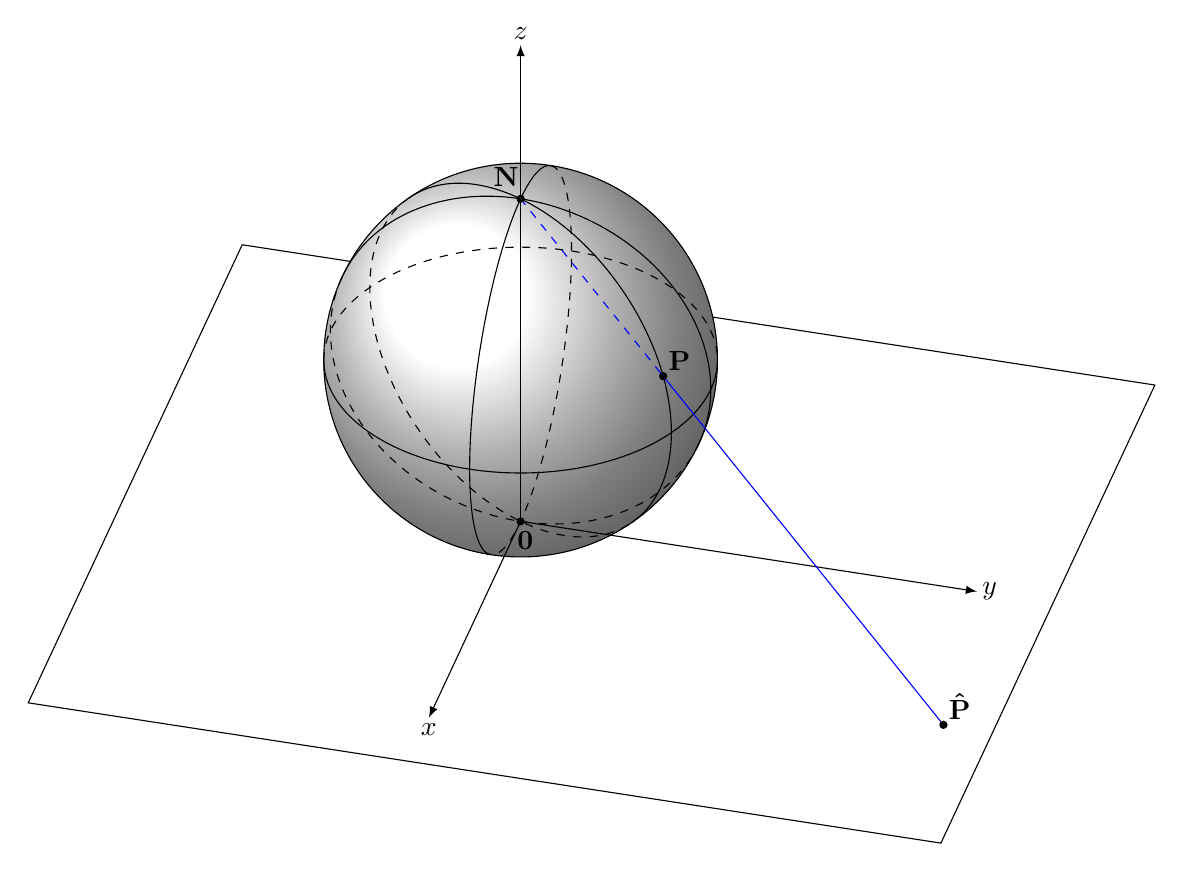
\begin{tikzpicture} % CENT
\newcommand\pgfmathsinandcos[3]{%
  \pgfmathsetmacro#1{sin(#3)}%
  \pgfmathsetmacro#2{cos(#3)}%
}
\newcommand\LongitudePlane[3][current plane]{%
  \pgfmathsinandcos\sinEl\cosEl{#2} % elevation
  \pgfmathsinandcos\sint\cost{#3} % azimuth
  \tikzset{#1/.estyle={cm={\cost,\sint*\sinEl,0,\cosEl,(0,0)}}}
}
\newcommand\LatitudePlane[3][current plane]{%
  \pgfmathsinandcos\sinEl\cosEl{#2} % elevation
  \pgfmathsinandcos\sint\cost{#3} % latitude
  \pgfmathsetmacro\yshift{\cosEl*\sint}
  \tikzset{#1/.estyle={cm={\cost,0,0,\cost*\sinEl,(0,\yshift)}}} %
}
\newcommand\DrawLongitudeCircle[2][1]{
  \LongitudePlane{\angEl}{#2}
  \tikzset{current plane/.prefix style={scale=#1}}
   % angle of "visibility"
  \pgfmathsetmacro\angVis{atan(sin(#2)*cos(\angEl)/sin(\angEl))} %
  \draw[current plane] (\angVis:1) arc (\angVis:\angVis+180:1);
  \draw[current plane,dashed] (\angVis-180:1) arc (\angVis-180:\angVis:1);
}
\newcommand\DrawLatitudeCircle[2][1]{
  \LatitudePlane{\angEl}{#2}
  \tikzset{current plane/.prefix style={scale=#1}}
  \pgfmathsetmacro\sinVis{sin(#2)/cos(#2)*sin(\angEl)/cos(\angEl)}
  % angle of "visibility"
  \pgfmathsetmacro\angVis{asin(min(1,max(\sinVis,-1)))}
  \draw[current plane] (\angVis:1) arc (\angVis:-\angVis-180:1);
  \draw[current plane,dashed] (180-\angVis:1) arc (180-\angVis:\angVis:1);
}

\tikzset{%
  >=latex, % option for nice arrows
  inner sep=0pt,%
  outer sep=2pt,%
  mark coordinate/.style={inner sep=0pt,outer sep=0pt,minimum size=3pt,
    fill=black,circle}%
}
%% some definitions

\def\R{2.5} % sphere radius
\def\angEl{35} % elevation angle
\def\angAz{-105} % azimuth angle
\def\angPhi{-40} % longitude of point P
\def\angBeta{19} % latitude of point P

%% working planes

\pgfmathsetmacro\H{\R*cos(\angEl)} % distance to north pole
\tikzset{xyplane/.estyle={cm={cos(\angAz),sin(\angAz)*sin(\angEl),-sin(\angAz),
                              cos(\angAz)*sin(\angEl),(0,-\H)}}}
\LongitudePlane[xzplane]{\angEl}{\angAz}
\LongitudePlane[pzplane]{\angEl}{\angPhi}
\LatitudePlane[equator]{\angEl}{0}

%% draw xyplane and sphere

\draw[xyplane] (-2*\R,-2*\R) rectangle (2.2*\R,2.8*\R);
\fill[ball color=white] (0,0) circle (\R); % 3D lighting effect
\draw (0,0) circle (\R);

%% characteristic points

\coordinate (O) at (0,0);
\coordinate[mark coordinate] (N) at (0,\H);
\coordinate[mark coordinate] (S) at (0,-\H);
\path[pzplane] (\angBeta:\R) coordinate[mark coordinate] (P);
\path[pzplane] (\R,0) coordinate (PE);
\path[xzplane] (\R,0) coordinate (XE);
\path (PE) ++(0,-\H) coordinate (Paux); % to aid Phat calculation
\coordinate[mark coordinate] (Phat) at (intersection cs: first line={(N)--(P)},
                                        second line={(S)--(Paux)});

%% draw meridians and latitude circles

\DrawLatitudeCircle[\R]{0} % equator
\DrawLongitudeCircle[\R]{\angAz} % xzplane
\DrawLongitudeCircle[\R]{\angAz+90} % yzplane
\DrawLongitudeCircle[\R]{\angPhi} % pzplane

%% draw xyz coordinate system

\draw[xyplane,<->] (1.8*\R,0) node[below] {$x$} -- (0,0) -- (0,2.4*\R)
    node[right] {$y$};
\draw[->] (0,-\H) -- (0,1.6*\R) node[above] {$z$};

%% draw lines and put labels

\draw[blue,dashed] (P) -- (N) +(0.3ex,0.6ex) node[above left,black] {$\mathbf{N}$};
\draw[blue] (P) -- (Phat) node[above right,black] {$\mathbf{\hat{P}}$};
\path (S) +(0.4ex,-0.4ex) node[below] {$\mathbf{0}$};
\draw (P) node[above right] {$\mathbf{P}$};
\end{tikzpicture}
}
        \caption{Visualisierung der stereographischen Projektion}
        \label{fig:stereographic-projection}
    \end{figure}

    Sei $P = \begin{pmatrix}x_1\\ \vdots \\ x_{n+1}\end{pmatrix}$, so
    ist $x_{n+1} < 1$, also ist $L_P$ nicht parallel zu $H$. Also
    schneiden sich $L_P$ und $H$ in genau einem Punkt $\hat{P}$.

    Es gilt: $f$ ist bijektiv und die Umkehrabbildung ist ebenfalls
    stetig.    
\end{beispiel}
\index{Stetigkeit|)}
%%%%%%%%%%%%%%%%%%%%%%%%%%%%%%%%%%%%%%%%%%%%%%%%%%%%%%%%%%%%%%%%%%%%%
% Mitschrieb vom 31.10.2013                                         %
%%%%%%%%%%%%%%%%%%%%%%%%%%%%%%%%%%%%%%%%%%%%%%%%%%%%%%%%%%%%%%%%%%%%%
\section{Zusammenhang}\index{Zusammenhang|(}
\begin{definition}\xindex{zusammenhaengend@zusammenhängend}%
    Ein Raum $X$ heißt \textbf{zusammenhängend}, wenn es keine offenen,
    nichtleeren Teilmengen $U_1, U_2$ von $X$ gibt mit 
    $U_1 \cap U_2 = \emptyset$ und $U_1 \cup U_2 = X$.
\end{definition}

\begin{bemerkung}
    $X$ ist zusammenhängend $\gdw$ Es gibt keine abgeschlossenen,
    nichtleeren Teilmengen $A_1, A_2$ mit $A_1 \cap A_2 = \emptyset$ 
    und $A_1 \cup A_2 = X$.
\end{bemerkung}

\begin{bemerkung}
    Eine Teilmenge $Y \subseteq X$ heißt zusammenhängend, wenn $Y$
    als topologischer Raum mit der Teilraumtopologie zusammenhängend ist.
\end{bemerkung}

%\begin{beispiel}
%
%\end{beispiel}

\begin{beispiel}[Zusammenhang von Räumen]
    \begin{bspenum}
        \item $\mdr^n$ ist mit der euklidischen Topologie zusammenhängend,
            denn:

            \underline{Annahme}: $\mdr^n = U_1 \cup U_2$ mit $U_i$ 
            offen, $U_i \neq \emptyset$ und $U_1 \cap U_2 = \emptyset$ 
            existieren.

            Sei $x \in U_1, y \in U_2$ und $[x,y]$ die Strecke zwischen $x$
            und $y$. Dann ist $U_1 \cap [x,y]$ die Vereinigung von offenen
            Intervallen. Dann gibt es $z \in [x,y]$ mit $z \in \partial (U_1 \cap [x,y])$,
            aber $z \notin U_1 \Rightarrow z \in U_2$. In jeder Umgebung von 
            $z$ liegt ein Punkt von $U_1 \Rightarrow$ Widerspruch zu $U_2$ offen.
        \item $\mdr \setminus \Set{0}$ ist nicht zusammenhängend, denn
              $\mdr \setminus \Set{0} = \mdr_{< 0} \cup \mdr_{> 0}$
        \item $\mdr^2 \setminus \Set{0}$ ist zusammenhängend.
        \item $\mdq \subsetneq \mdr$ ist nicht zusammenhängend, da 
              $(\mdq \cap \mdr_{< \sqrt{2}}) \cup (\mdq \cap \mdr_{> \sqrt{2}}) = \mdq$
        \item $\Set{x}$ ist zusammenhängend für jedes $x \in X$, 
              wobei $X$ ein topologischer Raum ist.
        \item $\mdr$ mit Zariski-Topologie ist zusammenhängend.\xindex{Topologie!Zariski}
    \end{bspenum}
\end{beispiel}

\begin{bemerkung}\label{zusammenhangAbschluss}
    Sei $X$ ein topologischer Raum und $A \subseteq X$ zusammenhängend.
    Dann ist auch $\overline{A}$ zusammenhängend.
\end{bemerkung}

\begin{beweis} durch Widerspruch\\
    \underline{Annahme}: $\overline{A} = A_1 \cup A_2,\; A_i$ abgeschlossen, $A_i \neq \emptyset$,
    $\;A_1 \cap A_2 = \emptyset$
    \begin{align*}
        &\Rightarrow A = \underbrace{\underbrace{(A \cap A_1)}_\text{abgeschlossen} \dcup \underbrace{(A \cap A_2)}_\text{abgeschlossen}}_\text{disjunkt}\\
    \end{align*}

    Wäre $A \cap A_1 = \emptyset$\\
    $\Rightarrow A \subseteq \overline{A} = A_1 \dcup A_2$\\
    $\Rightarrow A \subseteq A_2$
    $\Rightarrow \overline{A} \subseteq A_2$\\
    $\Rightarrow A_1 = \emptyset$\\
    $\Rightarrow$ Widerspruch zu $A_1 \neq \emptyset$\\
    $\Rightarrow A \cap A_1 \neq \emptyset$ und analog 
                $A \cap A_2 \neq \emptyset$\\
    $\Rightarrow$ Widerspruch zu $A$ ist zusammenhängend. $ \qed$
\end{beweis}

\begin{bemerkung}\label{bem:zusammenhangVereinigung}
    Sei $X$ ein topologischer Raum und $A, B \subseteq X$ zusammenhängend.

    Ist $A \cap B \neq \emptyset$, dann ist $A \cup B$ zusammenhängend.
\end{bemerkung}

\begin{beweis}
    Sei $A \cup B = U_1 \dcup U_2, U_i \neq \emptyset$ offen
    \begin{align*}
        &\xRightarrow{\text{\obda}} A = (A \cap U_1) \dcup (A \cap U_2) \text{ offen}\\
        &\xRightarrow{A \text{ zhgd.}} A \cap U_1 = \emptyset\\
        &\xRightarrow{A \cap B \neq \emptyset} U_1 \subseteq B\\
        &B = \underbrace{(B \cap U_1)}_{= U_1} \cup \underbrace{(B \cap U_2)}_{= \emptyset} \text{ ist unerlaubte Zerlegung.}
    \end{align*}
    $\qed$
\end{beweis}

\begin{definition}\xindex{Zusammenhangskomponente}%
    Sei $X$ ein topologischer Raum.
    
    Für $x \in X$ sei $Z(x) \subseteq X$ definiert durch
    \[Z(x) := \bigcup_{\mathclap{\substack{A \subseteq X \text{zhgd.}\\ x \in A}}} A\]

     $Z(x)$ heißt \textbf{Zusammenhangskomponente}.
\end{definition}

\begin{bemerkung}
    Sei $X$ ein topologischer Raum. Dann gilt:
    \begin{bemenum}
        \item $Z(X)$ ist die größte zusammenhängende Teilmenge von $X$,
              die $x$ enthält.
        \item $Z(X)$ ist abgeschlossen.
        \item $X$ ist disjunkte Vereinigung von Zusammenhangskomponenten.
    \end{bemenum}
\end{bemerkung}

\begin{beweis}\leavevmode
    \begin{enumerate}[label=\alph*)]
        \item Sei $Z(x) = A_1 \dcup A_2$ mit $A_i \neq \emptyset$ abgeschlossen.

            \Obda sei $x \in A_1$ und $y \in A_2$. $y$ liegt in einer zusammehängenden
            Teilmenge $A$, die auch $x$ enthält.
            $\Rightarrow A = \underbrace{(A \cap A_1)}_{\ni x} \cup \underbrace{(A \cap A_2)}_{\ni y}$
            ist unerlaubte Zerlegung.
        \item Nach \cref{zusammenhangAbschluss} ist $\overline{Z(x)}$
              zusammenhängend $\Rightarrow \overline{Z(x)} \subseteq Z(x)$
              $\Rightarrow Z(x) = \overline{Z(x)}$
        \item Ist $Z(y) \cap Z(x) \neq \emptyset \xRightarrow{\crefabbr{bem:zusammenhangVereinigung}} Z(y) \cup Z(x)$
              ist zusammenhängend. \\
              \begin{align*}
                \Rightarrow Z(x) \cup Z(y) &\subseteq Z(x) \Rightarrow Z(y) \subseteq Z(x)\\
                                           &\subseteq Z(y) \Rightarrow Z(x) \subseteq Z(y)
              \end{align*} 
    \end{enumerate}

    $\qed$
\end{beweis}

\begin{bemerkung}
    Sei $f:X \rightarrow Y$ stetig. Ist $A \subseteq X$ zusammenhängend,
    so ist $f(A) \subseteq Y$ zusammenhängend.
\end{bemerkung}

\begin{beweis}
    Sei $f(A) = U_1 \cup U_2, U_i \neq \emptyset,$ offen, disjunkt.

    $\Rightarrow f^{-1} (f(A)) = f^{-1}(U_1) \cup f^{-1}(U_2)$

    $\Rightarrow A = \underbrace{(A \cap f^{-1}(U_1))}_{\neq \emptyset} \cup \underbrace{(A \cap f^{-1}(U_2))}_{\neq \emptyset} \qed$
\end{beweis}\index{Zusammenhang|)}

\section{Kompaktheit}
\begin{definition}\xindex{Ueberdeckung@""Uberdeckung}%
    Sei $X$ eine Menge und $\fU \subseteq \powerset{X}$.

    $\fU$ heißt eine \textbf{Überdeckung} von $X$, wenn gilt:
    \[\forall x \in X: \exists M \in \fU: x \in M\]
\end{definition}

\begin{definition}\xindex{Raum!kompakter}%
    Ein topologischer Raum $X$ heißt \textbf{kompakt}, wenn jede
    offene Überdeckung von $X$
    \[\fU = \Set{U_i}_{i \in I} \text{ mit } U_i \text{ offen in } X\]
    eine endliche Teilüberdeckung 
    \[\bigcup_{\mathclap{i \in J \subseteq I}} U_i = X \text{ mit } |J| \in \mdn\]
    besitzt.
\end{definition}

%%%%%%%%%%%%%%%%%%%%%%%%%%%%%%%%%%%%%%%%%%%%%%%%%%%%%%%%%%%%%%%%%%%%%
% Mitschrieb vom 05.11.2013                                         %
%%%%%%%%%%%%%%%%%%%%%%%%%%%%%%%%%%%%%%%%%%%%%%%%%%%%%%%%%%%%%%%%%%%%%

\begin{bemerkung}\label{abgeschlossen01IstKompakt}
    Das Einheitsintervall $I := [0,1]$ ist kompakt bezüglich der 
    euklidischen Topologie.
\end{bemerkung}

\begin{beweis}
Sei $(U_i)_{i \in J}$ eine offene Überdeckung von $I$.

Es genügt zu zeigen, dass es ein $\delta > 0$ gibt, sodass jedes 
Teilintervall der Länge $\delta$ von $I$ in einem der $U_i$ enthalten ist.
Wenn es ein solches $\delta$ gibt, kann man $I$ in endlich viele 
Intervalle der Länge $\delta$ unterteilen und alle $U_i$ in die endliche
Überdeckung aufnehmen, die Teilintervalle enthalten.

Angenommen, es gibt kein solches $\delta$. Dann gibt es für jedes 
$n \in \mdn$ ein Intervall $I_n \subseteq [0,1]$ der Länge $\nicefrac{1}{n}$
sodass $I_n \subsetneq U_i$ für alle $i \in J$.

Sei $x_n$ der Mittelpunkt von $I_n$. Die Folge $(x_n)$ hat einen 
Häufungspunkt $x \in [0,1]$. Dann gibt es $i \in J$ mit $x \in U_i$.
Da $U_i$ offen ist, gibt es ein $\varepsilon > 0$, sodass $(x - \varepsilon, x + \varepsilon) \subseteq U_i$.
Dann gibt es $n_0$, sodass gilt:
$\nicefrac{1}{n_0} < \nicefrac{\varepsilon}{2}$ und für unendlich viele\footnote{Dies gilt nicht für alle $n \geq n_0$, da ein Häufungspunkt nur eine konvergente Teilfolge impliziert.}
$n\geq n_0: |x - x_n| < \nicefrac{\varepsilon}{2}$, also $I_n \subseteq (x - \varepsilon, x + \varepsilon) \subseteq U_i$
für mindestens ein $n \in \mdn$.\footnote{Sogar für unendlich viele.}

$\Rightarrow$ Widerspruch 

Dann überdecke $[0,1]$ mit endlich vielen Intervallen $I_1, \dots, I_d$
der Länge $\delta$. Jedes $I_j$ ist in $U_{ij}$ enthalten.

$\Rightarrow U_{j_1}, \dots, U_{j_d}$ ist endliche Teilüberdeckung von $U$.
$\qed$
\end{beweis}

\begin{beispiel}[Kompakte Räume]
    \begin{bspenum}
        \item $\mdr$ ist nicht kompakt.
        \item $(0,1)$ ist nicht kompakt.\\
              $U_n = (\nicefrac{1}{n}, 1-\nicefrac{1}{n}) \Rightarrow \bigcup_{n \in \mdn} U_n = (0,1)$
        \item $\mdr$ mit der Zariski-Topologie ist kompakt und jede 
              Teilmenge von $\mdr$ ist es auch.\xindex{Topologie!Zariski}
    \end{bspenum}
\end{beispiel}

\begin{bemerkung}\label{abgeschlossenInKomaktIstKompakt}
    Sei $X$ kompakter Raum, $A \subseteq X$ abgeschlossen. Dann ist
    $A$ kompakt.
\end{bemerkung}

\begin{beweis}
    Sei $(V_{i})_{i \in I}$ offene Überdeckung von A.\\
    Dann gibt es für jedes $i \in I$ eine offene Teilmenge $U_{i} \subseteq X$ mit $V_{i}=U_{i} \cap A$.
    \begin{align*}
        &\Rightarrow A \subseteq \bigcup_{i \in I} U_i\\
        &\Rightarrow \mathfrak{U} = \Set{U_i | i \in I} \cup \Set{X \setminus A} \text{ ist offene Überdeckung von } X\\
        &\xRightarrow{X \text{ kompakt}} \text{ es gibt } i_1, \dots, i_n \in I\text{, sodass }\bigcup_{j=1}^n U_{i_j} \cup (X \setminus A) = X\\
        &\Rightarrow \left (\bigcup_{j=1}^n U_{i_j} \cup (X \setminus A)\right ) \cap A = A\\
        &\Rightarrow \bigcup_{j=1}^n \underbrace{(U_{i_j} \cap A)}_{= V_{i_j}} \cup \underbrace{((X \setminus A) \cap A)}_{= \emptyset} = A\\
        &\Rightarrow V_{i_1}, \dots, V_{i_n} \text{ überdecken } A\text{.}
    \end{align*}
    $\qed$
\end{beweis}

\begin{bemerkung}\label{kompaktTimesKompaktIstKompakt}
    Seien $X, Y$ kompakte topologische Räume. Dann ist $X \times Y$
    mit der Produkttopologie kompakt.
\end{bemerkung}

\begin{beweis}
    Sei $(W_i)_{i \in I}$ eine offene Überdeckung von $X \times Y$.
    Für jedes $(x,y) \in X \times Y$ gibt es offene Teilmengen
    $U_{x,y}$ von $X$ und $V_{x,y}$ von $Y$ sowie ein $i \in I$, sodass
    $U_{x,y} \times V_{x,y} \subseteq W_i$.

    \begin{figure}[htp]
        \centering
        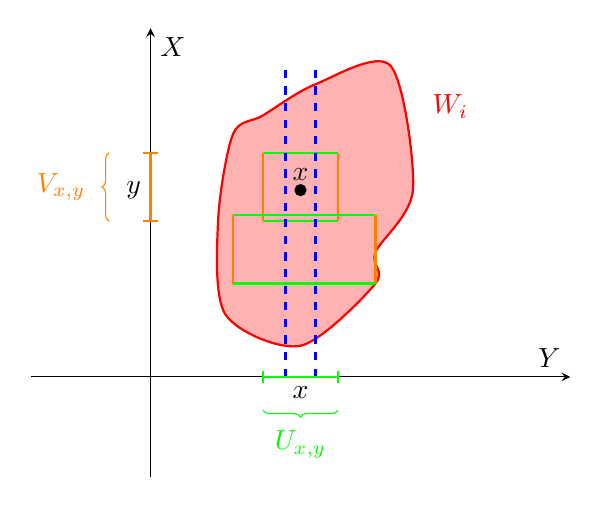
\begin{tikzpicture}
    \begin{axis}[
        axis x line=middle,
        axis y line=middle,
        %width=9cm,
        %height=4.5cm,
        xmin=-1,     % start the diagram at this x-coordinate
        xmax= 5,     % end   the diagram at this x-coordinate
        ymin=-1,     % start the diagram at this y-coordinate
        ymax= 5,     % end   the diagram at this y-coordinate
        xlabel=$Y$,
        ylabel=$X$,
        ticks=none,
        enlargelimits=true,
        after end axis/.code={
            \draw [decorate,decoration={brace,mirror,raise=15pt}, orange] (axis cs:0,3.6) -- (axis cs:0,2.5) node [midway,left=20pt,orange] {$V_{x,y}$};
            \draw [decorate,decoration={brace,mirror,raise=12pt}, green]  (axis cs:1.5,0) -- (axis cs:2.5,0) node [midway,below=16pt,green] {$U_{x,y}$};
        }]

        \addplot[mark=none, red, smooth cycle, thick, fill=red!30] coordinates {(1,1) (2,0.5) (3,1.5) (3,2) (3.5,3) (3.2, 5) (2.2, 4.7) (1.5, 4.2) (1.1, 3.9) (0.9, 2.5)};
        \node[red] at (axis cs:4,4) [anchor=south] {$W_i$};

        % Draw help lines
        %\addplot[dashed] coordinates {(1.5,0) (1.5,3.6)};
        %\addplot[dashed] coordinates {(2.5,0) (2.5,3.6)};
        %\addplot[dashed] coordinates {(0,2.5) (2.5,2.5)};
        %\addplot[dashed] coordinates {(0,3.6) (2.5,3.6)};

        % Draw solid square
        \addplot[mark=none, orange, thick] coordinates {(2.5,2.5) (2.5,3.6)};
        \addplot[mark=none, green, thick]  coordinates {(2.5,3.6) (1.5,3.6)};
        \addplot[mark=none, orange, thick] coordinates {(1.5,3.6) (1.5,2.5)};
        \addplot[mark=none, green, thick]  coordinates {(1.5,2.5) (2.5,2.5)};

        \addplot[mark=none, orange, thick] coordinates {(3.0,1.5) (3.0,2.6)};
        \addplot[mark=none, green, thick]  coordinates {(3.0,2.6) (1.1,2.6)};
        \addplot[mark=none, orange, thick] coordinates {(1.1,1.5) (1.1,2.6)};
        \addplot[mark=none, green, thick]  coordinates {(1.1,1.5) (3.0,1.5)};


        \addplot[mark=none, orange, thick] coordinates {(3.0,1.5) (3.0,2.6)};
        \addplot[mark=none, green, thick]  coordinates {(3.0,2.6) (1.1,2.6)};
        \addplot[mark=none, orange, thick] coordinates {(1.1,1.5) (1.1,2.6)};
        \addplot[mark=none, green, thick]  coordinates {(1.1,1.5) (3.0,1.5)};

        \addplot[mark=none, blue, thick, dashed]  coordinates {((1.8,0) (1.8,5)};
        \addplot[mark=none, blue, thick, dashed]  coordinates {((2.2,0) (2.2,5)};

        % Draw x and annotation
        \node at (axis cs:2,3) [anchor=-90] {$x$};
        \addplot[mark=*] coordinates {(2,3)};

        % Draw ticks of help lines
        \addplot[mark=none, green, thick] coordinates {(1.5, -0.1) (1.5,0.1)};
        \addplot[mark=none, green, thick] coordinates {(2.5, -0.1) (2.5,0.1)};
        \addplot[mark=none, green, thick] coordinates {(1.5, 0) (2.5,0)};

        \addplot[mark=none, orange, thick] coordinates {(-0.1, 2.5) (0.1,2.5)};
        \addplot[mark=none, orange, thick] coordinates {(-0.1, 3.6) (0.1,3.6)};
        \addplot[mark=none, orange, thick] coordinates {(0, 2.5) (0,3.6)};

        % Draw axis text
        \node at (axis cs:0,3) [anchor=east] {$y$};
        \node at (axis cs:2,0) [anchor=north] {$x$};

    \end{axis} 
\end{tikzpicture}

        \caption{Die blaue Umgebung ist Schnitt vieler Umgebungen}
    \end{figure}

    Die offenen Mengen $U_{x_0, y} \times V_{x_0, y}$ für festes $x_0$
    und alle $y \in Y$ überdecken $\Set{x_0} \times y$. Da $Y$ kompakt
    ist, ist auch $\Set{x_0} \times Y$ kompakt. Also gibt es 
    $y_1, \dots, y_{m(x_0)}$ mit 
    $\bigcup_{i=1}^{m(x_0)} U_{x_0, y_i} \times V_{x_0, y_i} \supseteq \Set{x_0} \times Y$.

    Sei ${\color{blue} U_{x_0}} := \bigcap_{i=1}^{m(x)} U_{x_0, y_i}$.
    Da $X$ kompakt ist, gibt es $x_1, \dots, x_n \in X$ mit 
    $\bigcup_{j=1}^n U_{x_j} = X$\\
    $\Rightarrow \bigcup_{j=1}^k \bigcup_{i=1}^{m(x_j)} \underbrace{\left ( U_{x_j, y_i} \times V_{x_j, y_i} \right)}_{\text{Ein grün-oranges Kästchen}} \supseteq X \times Y$\\
    $\Rightarrow \bigcup_j \bigcup_i W_i (x_j, y_i) = X \times Y \qed$
\end{beweis}

\begin{bemerkung}\label{hausdorffraumKompakteTeilmengeAbgeschlossen}
    Sei $X$ ein Hausdorffraum und $K \subseteq X$ kompakt.
    Dann ist $K$ abgeschlossen.
\end{bemerkung}

\begin{beweis}
    \underline{z.~Z.:} Komplement ist offen

    Ist $X = K$, so ist $K$ abgeschlossen in $X$. Andernfalls sei 
    $y \in X \setminus K$. Für jedes $x \in K$ seien $U_x$ bzw. $V_y$
    Umgebungen von $x$ bzw. von $y$, sodass $U_x \cap V_y = \emptyset$.

    \begin{figure}[htp]
        \centering
        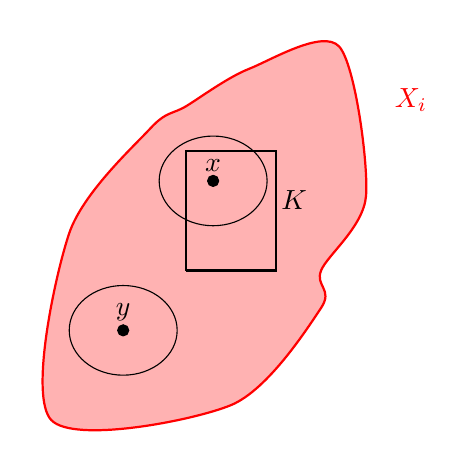
\begin{tikzpicture}
    \begin{axis}[
        axis x line=none,
        axis y line=none,
        %width=9cm,
        %height=4.5cm,
        xmin= 0,     % start the diagram at this x-coordinate
        xmax= 5,     % end   the diagram at this x-coordinate
        ymin= 0,     % start the diagram at this y-coordinate
        ymax= 5,     % end   the diagram at this y-coordinate
        xlabel=$Y$,
        ylabel=$X$,
        ticks=none,
        enlargelimits=true]

        \addplot[mark=none, red, smooth cycle, thick, fill=red!30] coordinates {(0,0) (2,0.2) (3,1.5) (3,2) (3.5,3) (3.2, 5) (2.2, 4.7) (1.5, 4.2) (1.1, 3.9) (0.2, 2.5)};
        \node[red] at (axis cs:4,4) [anchor=south] {$X_i$};

        % Draw solid square
        \addplot[mark=none, thick] coordinates {(1.5,2.0) (2.5,2.0) (2.5,3.6) (1.5,3.6) (1.5,2.0)};
        \node at (axis cs:2.7,3.2) [anchor=90] {$K$};


        % Draw x and annotation
        \node at (axis cs:1.8,3.2) [anchor=-90] {$x$};
        \draw (axis cs:1.8,3.2) circle[radius=0.6];
        \addplot[mark=*] coordinates {(1.8,3.2)};

        \node at (axis cs:0.8,1.2) [anchor=-90] {$y$};
        \draw (axis cs:0.8,1.2) circle[radius=0.6];
        \addplot[mark=*] coordinates {(0.8,1.2)};
    \end{axis}
\end{tikzpicture}

    \end{figure}

    Da $K$ kompakt ist, gibt es endlich viele $x_1, \dots, x_n \in K$,
    sodass $\bigcup_{i=1}^m U_{x_i} \supseteq K$.

    \begin{align*}
        &\text{Sei } V := \bigcap_{i=1}^n V_{x_i}\\
        &\Rightarrow V \cap \left (\bigcup_{i=1}^n U_{x_i} \right) = \emptyset \\
        &\Rightarrow V \cap K = \emptyset\\
        &\Rightarrow V \text{ ist Überdeckung von } y\text{, die ganz in } X \setminus K \text{ enthalten ist}.\\
        &\Rightarrow X \setminus K \text{ ist offen}
    \end{align*}
    Damit ist $K$ abgeschlossen. $\qed$
\end{beweis}

\begin{bemerkung}\label{kor:5.6}%In Vorlesung: Bemerkung 5.6
    Seien $X, Y$ topologische Räume, $f: X \rightarrow Y$ stetig.
    Ist $K \subseteq X$ kompakt, so ist $f(K) \subseteq Y$ kompakt.
\end{bemerkung}

\begin{beweis}
    Sei $(V_i)_{i \in I}$ offene Überdeckung von $f(K)$\\
    $\xRightarrow{f \text{ stetig}} (f^{-1}(V_i))_{i \in I}$ ist offene Überdeckung von $K$\\
    $\xRightarrow{\text{Kompakt}}$ es gibt $i_1, \dots, i_n$, 
    sodass $f^{-1}(V_{i_1}), \dots, f^{-1}(V_{i_n})$ Überdeckung von
    $K$ ist.\\
    $\Rightarrow f(f^{-1}( V_{i_1})), \dots, f(f^{-1}(V_{i_n}))$ 
    überdecken $f(K)$.

    Es gilt: $f(f^{-1}(V)) = V \cap f(X) \qed$
\end{beweis}

\begin{satz}[Heine-Borel]\label{satz:heine-borel}%In Vorlesung: Proposition 5.7
    Eine Teilmenge von $\mdr^n$ oder $\mdc^n$ ist genau dann kompakt,
    wenn sie beschränkt und abgeschlossen ist.
\end{satz}

\begin{beweis}\leavevmode
    \enquote{$\Rightarrow$}: Sei $K \subseteq \mdr^n$ (oder $\mdc^n$)
    kompakt.

    Da $\mdr^n$ und $\mdc^n$ hausdorffsch sind, ist $K$ nach
    \cref{hausdorffraumKompakteTeilmengeAbgeschlossen} abgeschlossen.
    Nach Voraussetzung kann $K$ mit endlich vielen offenen Kugeln von 
    Radien 1 überdeckt werden $\Rightarrow K$ ist beschränkt.

    \enquote{$\Leftarrow$} Sei $A \subseteq \mdr^n$ (oder $\mdc^n$)
    beschränkt und abgeschlossen.

    Dann gibt es einen Würfel $W = \underbrace{[-N, N] \times \dots \times [-N, N]}_{n \text{ mal}}$
    mit $A \subseteq W$ bzw. \enquote{Polyzylinder}\xindex{Polyzylinder}
    $Z = \Set{(z_1, \dots, z_n) \in \mdc^n | z_i \leq N \text{ für } i= 1, \dots, n}$

    Nach \cref{kompaktTimesKompaktIstKompakt} und
    \cref{abgeschlossen01IstKompakt} ist $W$ kompakt, also ist $A$
    nach \cref{abgeschlossenInKomaktIstKompakt} auch kompakt.
    Genauso ist $Z$ kompakt, weil 
    \[\Set{z \in \mdc | |z| \leq 1}\]
    homöomorph zu
    \[\Set{(x,y) \in \mdr^2 | \|(x,y)\| \leq 1}\]
    ist. $\qed$
\end{beweis}

%%%%%%%%%%%%%%%%%%%%%%%%%%%%%%%%%%%%%%%%%%%%%%%%%%%%%%%%%%%%%%%%%%%%%
% Mitschrieb vom 07.11.2013                                         %
%%%%%%%%%%%%%%%%%%%%%%%%%%%%%%%%%%%%%%%%%%%%%%%%%%%%%%%%%%%%%%%%%%%%%
\section{Wege und Knoten}\index{Knoten|(}
\begin{definition}\xindex{Weg}\xindex{Weg!geschlossener}\xindex{Weg!einfacher}%
    Sei $X$ ein topologischer Raum. 
    \begin{defenum}
        \item Ein \textbf{Weg} in $X$ ist eine stetige Abbildung $\gamma:[0,1] \rightarrow X$.
        \item $\gamma$ heißt \textbf{geschlossen}, wenn $\gamma(1) = \gamma(0)$ gilt.
        \item $\gamma$ heißt \textbf{einfach}, wenn $\gamma|_{[0,1)}$ 
              injektiv ist.
    \end{defenum}
\end{definition}

\begin{beispiel}
    Ist $X$ diskret, so ist jeder Weg konstant, d.~h. von der Form
    \[\forall x \in [0,1]: \gamma(x) = c, \;\;\; c \in X\]
    Denn $\gamma([0,1])$ ist zusammenhängend für jeden Weg $\gamma$.
\end{beispiel}

\begin{definition}\xindex{Wegzusammenhang}%
    Ein topologischer Raum $X$ heißt \textbf{wegzusammenhängend},
    wenn es zu je zwei Punkten $x,y \in X$ einen Weg $\gamma:[0,1] \rightarrow X$
    gibt mit $\gamma(0)=x$ und $\gamma(1)=y$.
\end{definition}

\begin{bemerkung}\label{kor:wegzusammehang-impliziert-zusammenhang}
    Sei $X$ ein topologischer Raum.

    \begin{bemenum}
        \item $X$ ist wegzusammenhängend $\Rightarrow X$ ist zusammenhängend
        \item $X$ ist wegzusammenhängend $\not\Leftarrow X$ ist zusammenhängend
    \end{bemenum}
\end{bemerkung}

\begin{beweis}\leavevmode
    \begin{enumerate}[label=\alph*)]
    \item Sei $X$ ein wegzusammenhängender topologischer Raum, $A_1, A_2$
    nichtleere, disjunkte, abgeschlossene Teilmengen von $X$ mit
    $A_1 \cup A_2 = X$. Sei $x \in A_1, y \in A_2, \gamma:[0,1] \rightarrow X$
    ein Weg von $x$ nach $y$.

    Dann ist $C:= \gamma([0,1]) \subseteq X$ zusammenhängend, weil 
    $\gamma$ stetig ist.
    \[C = \underbrace{(C \cap A_1)}_{\ni x} \cup \underbrace{(C \cap A_2)}_{\ni y}\]
    ist Zerlegung in nichtleere, disjunkte, abgeschlossene Teilmengen
    $\Rightarrow$ Widerspruch 

    \item Sei $X = \Set{(x,y) \in \mdr^2| x^2 + y^2 = 1 \lor y = 1 +2\cdot e^{-\frac{1}{10} x}}$.

        \Cref{fig:topology-spiral} veranschaulicht diesen Raum.

        \begin{figure}[htp]
            \centering
            \subfloat[Spirale $S$ mit Kreis $C$]{
                \resizebox{0.25\linewidth}{!}{% Thanks to Jake: http://tex.stackexchange.com/a/142815/5645
\documentclass[border=5pt]{standalone}
\usepackage{tikz}
\usetikzlibrary{arrows}

\begin{document}
\begin{tikzpicture}
    \draw [red] (0,0) circle [radius=1];
    \draw [domain=1:18.8,variable=\t,smooth,samples=200,->,>=stealth']
        plot ({\t r}: {1+2*exp(-0.1*\t)});
\end{tikzpicture}
\end{document}
}
                \label{fig:topology-spiral}
            }%
            \subfloat[Sinus]{
                \resizebox{0.65\linewidth}{!}{\documentclass{article}
\usepackage[pdftex,active,tightpage]{preview}
\setlength\PreviewBorder{2mm}

\usepackage{pgfplots}
\pgfplotsset{compat=1.9}
\usepackage{tikz}
\usetikzlibrary{arrows, positioning, calc}

\begin{document}
\begin{preview}

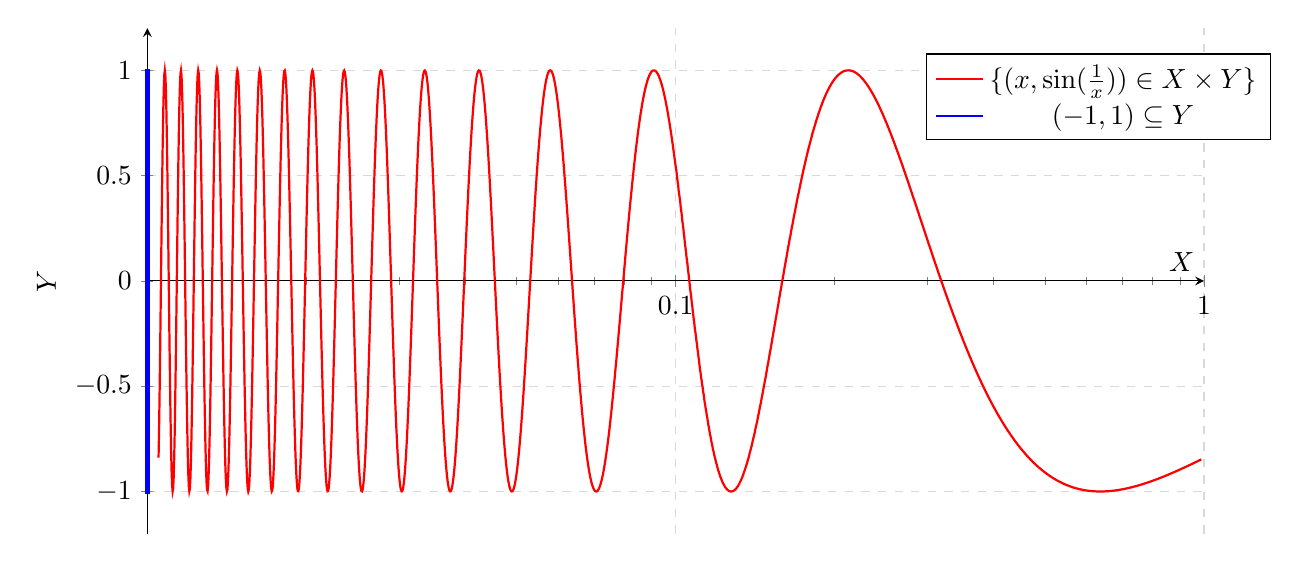
\begin{tikzpicture}
    \begin{axis}[
        axis x line=middle,
        axis y line=left,
        enlarge y limits=true,
        xmode=log, % Logarithmic x axis
        xmin=0.01, xmax=1, % Positive domain...
        xticklabel=\pgfmathparse{exp(\tick)}\pgfmathprintnumber{\pgfmathresult},
        xticklabel style={/pgf/number format/.cd,fixed}, % Use fixed point notation
        width=15cm, height=8cm,     % size of the image
        grid = major,
        grid style={dashed, gray!30},
        ymin=-1,      % start the diagram at this y-coordinate
        ymax= 1,      % end   the diagram at this y-coordinate
        axis background/.style={fill=white},
        ylabel=$Y$,
        xlabel=$X$,
        legend style={at={(0.9,0.95)}, anchor=north}
     ]
      \addplot[domain=0.0105:1, red, thick,samples=2000] {-sin(deg(1/(x)))};
      \addplot[domain=0.0105:0.011, blue, thick,samples=20] {10};
      \addlegendentry{$\{(x, \sin(\frac{1}{x})) \in X \times Y\}$}
      \addlegendentry{$(-1,1) \subseteq Y$}
    \end{axis}
      \draw[ultra thick,blue] (0,0.5) -- (0,5.9);
\end{tikzpicture}
\end{preview}
\end{document}
}
                \label{fig:sinx}
            }%

            \caption{Beispiele für Räume, die zusammenhängend, aber nicht wegzusammenhängend sind.}
            \label{fig:zusammenhang-beispiele}
        \end{figure}

          Sei $U_1 \cup U_2 = X, U_1 \neq U_2 = \emptyset, U_i$ offen.
          $X = C \cup S$. Dann ist $C \subseteq U_1$ oder $C \subseteq U_2$,
          weil $C$ und $S$ zusammenhängend sind.

          Also ist $C = U_1$ und $S = U_2$ (oder umgekehrt).

          Sei $y \in C = U_1, \varepsilon > 0$ und $\fB_\varepsilon (y) \subseteq U_1$
          eine Umgebung von $y$, die in $U_1$ enthalten ist.

          Aber: $\fB_\varepsilon(y) \cap S \neq \emptyset \Rightarrow$
          Widerspruch $\Rightarrow X \cup S$ ist zusammenhängend, aber
          nicht wegzusammenhängend.
$\qed$
    \end{enumerate}
\end{beweis}

\begin{beispiel}[Hilbert-Kurve]\xindex{Hilbert-Kurve}%
    Es gibt stetige, surjektive Abbildungen 
    $[0,1] \rightarrow [0,1] \times [0,1]$. Ein Beispiel ist die
    in \cref{fig:hilbert-curve} dargestellte Hilbert-Kurve.

    % Author: Marc van Dongen
% Source: http://www.texample.net/tikz/examples/hilbert-curve/
\newdimen\HilbertLastX
\newdimen\HilbertLastY
\newcounter{HilbertOrder}

\def\DrawToNext#1#2{%
   \advance \HilbertLastX by #1
   \advance \HilbertLastY by #2
   \pgfpathlineto{\pgfqpoint{\HilbertLastX}{\HilbertLastY}}
   % Alternative implementation using plot streams:
   % \pgfplotstreampoint{\pgfqpoint{\HilbertLastX}{\HilbertLastY}}
}

% \Hilbert[right_x,right_y,left_x,left_x,up_x,up_y,down_x,down_y]
\def\Hilbert[#1,#2,#3,#4,#5,#6,#7,#8] {
  \ifnum\value{HilbertOrder} > 0%
     \addtocounter{HilbertOrder}{-1}
     \Hilbert[#5,#6,#7,#8,#1,#2,#3,#4]
     \DrawToNext {#1} {#2}
     \Hilbert[#1,#2,#3,#4,#5,#6,#7,#8]
     \DrawToNext {#5} {#6}
     \Hilbert[#1,#2,#3,#4,#5,#6,#7,#8]
     \DrawToNext {#3} {#4}
     \Hilbert[#7,#8,#5,#6,#3,#4,#1,#2]
     \addtocounter{HilbertOrder}{1}
  \fi
}


% \hilbert((x,y),order)
\def\hilbert((#1,#2),#3){%
   \advance \HilbertLastX by #1
   \advance \HilbertLastY by #2
   \pgfpathmoveto{\pgfqpoint{\HilbertLastX}{\HilbertLastY}}
   % Alternative implementation using plot streams:
   % \pgfplothandlerlineto
   % \pgfplotstreamstart
   % \pgfplotstreampoint{\pgfqpoint{\HilbertLastX}{\HilbertLastY}}
   \setcounter{HilbertOrder}{#3}
   \Hilbert[1mm,0mm,-1mm,0mm,0mm,1mm,0mm,-1mm]
   \pgfusepath{stroke}%
}

\begin{figure}[htp]%
    \centering
    % draw Hilbert curves of order n=1,...,5
    % Warning! Curves with order > 6 may crash TeX
    \subfigure[$n=1$]{\tikz[scale=18] \hilbert((0mm,0mm),1);}~~
    \subfigure[$n=2$]{\tikz[scale=6] \hilbert((0mm,0mm),2);}~~
    \subfigure[$n=3$]{\tikz[scale=2.6] \hilbert((0mm,0mm),3);}~~
    \subfigure[$n=4$]{\tikz[scale=1.2] \hilbert((0mm,0mm),4);}~~
    \subfigure[$n=5$]{\tikz[scale=0.58] \hilbert((0mm,0mm),5);}%
    \caption{Hilbert-Kurve}\xindex{Hilbert-Kurve}
    \label{fig:hilbert-curve}
\end{figure}%

\end{beispiel}

\begin{definition}\xindex{Jordankurve}\xindex{Jordankurve!geschlossene}%
    Sei $X$ ein topologischer Raum. Eine (geschlossene)
    \textbf{Jordankurve} in $X$ ist ein Homöomorphismus 
    $\gamma: [0,1] \rightarrow C \subseteq X$ bzw.
    $\gamma: S^1 \rightarrow C \subseteq X$.
\end{definition}

\begin{satz}[Jordanscher Kurvensatz]
    Ist $C=\gamma([0,1])$ eine geschlossene Jordankurve in $\mdr^2$,
    so hat $\mdr^2 \setminus C$ genau zwei Zusammenhangskomponenten,
    von denen eine beschränkt ist und eine unbeschränkt.
\end{satz}

\begin{figure}[htp]
    \centering
    \documentclass[varwidth=true, border=2pt]{standalone}
\usepackage{tikz}
\usetikzlibrary{patterns,calc}
\usepackage{pgfplots}
\pgfplotsset{compat=1.7}

\begin{document}
% Code from Christian Feuersänger
% http://tex.stackexchange.com/questions/54794/using-a-pgfplots-style-legend-in-a-plain-old-tikzpicture#54834
% argument #1: any options
\newenvironment{customlegend}[1][]{%
    \begingroup
    % inits/clears the lists (which might be populated from previous
    % axes):
    \csname pgfplots@init@cleared@structures\endcsname
    \pgfplotsset{#1}%
}{%
    % draws the legend:
    \csname pgfplots@createlegend\endcsname
    \endgroup
}%

% makes \addlegendimage available (typically only available within an
% axis environment):
\def\addlegendimage{\csname pgfplots@addlegendimage\endcsname}

%%--------------------------------

% definition to insert numbers
\pgfkeys{/pgfplots/number in legend/.style={%
        /pgfplots/legend image code/.code={%
            \node at (0.295,-0.0225){#1};
        },%
    },
}
\begin{tikzpicture}
    \draw[draw=white,pattern=north west lines, pattern color=blue] (-1.5,-1.5) rectangle (1.5,1.5);
    \draw[fill=white] (0cm,0cm) circle(1cm);
    \draw[fill=white,thick,pattern=dots, pattern color=red] (0cm,0cm) circle(1cm);

    \begin{customlegend}[
    legend entries={ % <= in the following there are the entries
    au{\ss}en,
    innen,
    Jordankurve
    },
    legend style={at={(4.5,1.5)},font=\footnotesize}] % <= to define position and font legend
    % the following are the "images" and numbers in the legend
        \addlegendimage{area legend,pattern=north west lines, pattern color=blue,draw=white}
        \addlegendimage{area legend,pattern=dots, pattern color=red,draw=white}
        \addlegendimage{thick}
    \end{customlegend}
\end{tikzpicture}
\end{document}
 
    \label{fig:jordan-kurvensatz}
    \caption{Die unbeschränkte Zusammenhangskomponente wird häufig inneres, die beschränkte äußeres genannt.}
\end{figure}

\begin{beweis}
    ist technisch mühsam und wird hier nicht geführt. Er kann
    in \enquote{Algebraische Topologie: Eine Einführung} von R.~Stöcker
    und H.~Zieschang auf S. 301f (ISBN 978-3519122265) nachgelesen werden.

    Idee: Ersetze Weg $C$ durch Polygonzug.
\end{beweis}

\begin{definition}\xindex{Knoten}%
    Eine geschlossene Jordankurve in $\mdr^3$ heißt \textbf{Knoten}.
\end{definition}

\begin{beispiel}[Knoten]
    \xindex{Kleeblattknoten}\xindex{Achterknoten}\xindex{Knoten!trivialer}
    \begin{figure}[htp]
        \centering
        \subfloat[Trivialer Knoten]{
            \includegraphics[width=0.2\linewidth, keepaspectratio]{figures/blue-unknot.png}
            \label{fig:knot-unknot}
        }%
        \subfloat[Kleeblattknoten]{
            \includegraphics[width=0.2\linewidth, keepaspectratio]{figures/blue-trefoil-knot.png} 
            \label{fig:knot-trefoil}
        }%
        \subfloat[Achterknoten]{
            \includegraphics[width=0.2\linewidth, keepaspectratio]{figures/blue-eight-knot.png} 
            \label{fig:knot-eight-knot}
        }%
        \subfloat[$6_2$-Knoten]{
            \includegraphics[width=0.2\linewidth, keepaspectratio]{figures/blue-6-2-knot.png} 
            \label{fig:knot-6-2}
        }

        \caption{Beispiele für verschiedene Knoten}
        \label{fig:Knoten}
    \end{figure}
\end{beispiel}

\begin{definition}\xindex{Knoten!äquivalente}\xindex{Isotopie}%
    Zwei Knoten $\gamma_1, \gamma_2: S^1 \rightarrow \mdr^3$ heißen
    \textbf{äquivalent}, wenn es eine stetige Abbildung
    \[H: S^1 \times [0,1] \rightarrow \mdr^3\]
    gibt mit 
    \begin{align*}
        H(z,0) &= \gamma_1(z)\\
        H(z,1) &= \gamma_2(z)
    \end{align*}
    und für jedes
    feste $t \in [0,1]$ ist 
    \[H_z: S^1 \rightarrow \mdr^3, z \mapsto H(z,t)\]
    ein Knoten. Die Abbildung $H$ heißt \textbf{Isotopie} zwischen
    $\gamma_1$ und $\gamma_2$.
\end{definition}

\begin{definition}\xindex{Knotendiagramm}%
    Ein \textbf{Knotendiagramm} eines Knotens $\gamma$ ist eine 
    Projektion $\pi: \mdr^3 \rightarrow E$ auf eine Ebene $E$, sodass
    $|(\pi|C)^{-1}(x)| \leq 2$ für jedes $x \in D$.

    Ist $(\pi|C)^{-1}(x) = \Set{y_1, y_2}$, so \textbf{liegt $y_1$ über $y_2$},
    wenn $(y_1-x) = \lambda (y_2 - x)$ für ein $\lambda > 1$ ist.
\end{definition}

\begin{satz}[Satz von Reidemeister]
    Zwei endliche Knotendiagramme gehören genau dann zu äquivalenten
    Knoten, wenn sie durch endlich viele \enquote{Reidemeister-Züge}
    ineinander überführt werden können.
\end{satz}

\begin{figure}[htp]
    \centering
    \subfloat[$\Omega_1$]{
        \includegraphics[height=0.2\linewidth, keepaspectratio]{figures/reidemeister-move-1.png} 
        \label{fig:reidemeister-1}
    }\qquad\qquad%
    \subfloat[$\Omega_2$]{
        \includegraphics[height=0.2\linewidth, keepaspectratio]{figures/reidemeister-move-2.png} 
        \label{fig:reidemeister-2}
    }

    \subfloat[$\Omega_3$]{
        \includegraphics[height=0.2\linewidth, keepaspectratio]{figures/reidemeister-move-3.png} 
        \label{fig:reidemeister-3}
    }

    \caption{Reidemeister-Züge}
    \label{fig:reidemeister-zuege}
\end{figure}

\begin{beweis}
    Durch sorgfältige Fallunterscheidung.\footnote{Siehe \enquote{Knot Theory and Its Applications} von Kunio Murasugi. ISBN 978-0817638177.}
\end{beweis}

\begin{definition}\xindex{Färbbarkeit}%
    Ein Knotendiagramm heißt \textbf{3-färbbar}, 
    wenn jeder Bogen von $D$ so mit einer Farbe gefärbt werden kann, 
    dass an jeder Kreuzung eine oder 3 Farben auftreten und alle 3 
    Farben auftreten.
\end{definition}

\begin{figure}[htp]
    \centering
    \includegraphics[height=0.3\linewidth, keepaspectratio]{figures/tricoloring.png} 

    \caption{Ein 3-gefärber Kleeblattknoten}
    \label{fig:treefoil-knot-three-colors}
\end{figure}
\index{Knoten|)}

% Die Übungsaufgaben sollen ganz am Ende des Kapitels sein.
\clearpage
\section*{Übungsaufgaben}
\addcontentsline{toc}{section}{Übungsaufgaben}

\begin{aufgabe}[Sierpińskiraum]\label{ub1:aufg1}\xindex{Sierpińskiraum}
    Es sei $X := \Set{0,1}$ und $\fT_X := \Set{\emptyset, \Set{0}, X}$.
    Dies ist der sogenannte Sierpińskiraum.
    \begin{enumerate}[label=(\alph*)]
        \item Beweisen Sie, dass $(X, \fT_X)$ ein topologischer Raum ist.
        \item Ist $(X, \fT_X)$ hausdorffsch?
        \item Ist $\fT_X$ von einer Metrik erzeugt?
    \end{enumerate}
\end{aufgabe}

\begin{aufgabe}\label{ub1:aufg4}
    Es sei $\mdz$ mit der von den Mengen $U_{a,b} := a + b \mdz (a \in \mdz, b \in \mdz \setminus \Set{0})$
    erzeugten Topologie versehen.

    Zeigen Sie:
    \begin{enumerate}[label=(\alph*)]
        \item Jedes $U_{a,b}$ und jede einelementige Teilmenge von $\mdz$ ist abgeschlossen.
        \item $\Set{-1, 1}$ ist nicht offen.
        \item Es gibt unendlich viele Primzahlen.
    \end{enumerate}
\end{aufgabe}

\begin{aufgabe}[Cantorsches Diskontinuum]\label{ub2:aufg4}\xindex{Cantorsches Diskontinuum}
    Für jedes $i \in \mdn$ sei $P_i := \Set{0,1}$ mit der diskreten
    Topologie. Weiter Sei $P := \prod_{i \in \mdn} P_i$.

    \begin{enumerate}[label=(\alph*)]
        \item Wie sehen die offenen Mengen von $P$ aus?
        \item Was können Sie über den Zusammenhang von $P$ sagen?
    \end{enumerate}
\end{aufgabe}

\begin{aufgabe}[Kompaktheit]\label{ub3:aufg1}
    \begin{enumerate}[label=(\alph*)]
        \item Ist $\GL_n(\mdr) = \Set{A \in \mdr^{n \times n} | \det(A) \neq 0}$ kompakt?\xindex{Gruppe!allgemeine lineare}
        \item Ist $\SL_n(\mdr) = \Set{A \in \mdr^{n \times n} | \det(A) = 1}$ kompakt?\xindex{Gruppe!spezielle lineare}
        \item Ist $\praum(\mdr)$ kompakt?\xindex{Raum!projektiver}
    \end{enumerate}
\end{aufgabe}

